\chapter{Introduction}
\label{chap:introduction}

Introductory text -> Motivation for\\
- time variation analysis\\
- distance analysis\\
- Kp impact analysis\\
%(Kurzer Text zur Motivation für diese Arbeit, wie das Ziel erreicht wurde und wie es zum Thema kam.)

% Questions this work asks:\\	%Fragestellungen ausformuliert
% 	How strong is the solar wind influence on the terrestrial magnetosphere?\\
% 	How often occur certain solar wind ranges?\\
% 	How strong do different structure types influence the terrestrial magnetosphere?\\
% forecast:\\
% 	How can the impact strength of the solar wind be forecasted? (VBz->Kp L1-Alerts)\\
% 	How can the impact strength of CMEs be forecasted (V->Kp correlation for CMEs)?\\
% 	(How can the impact field strength of CMEs be forecasted (V->B correlation for CMEs)?)\\

% 	How does the solar wind evolve on its way from the Sun?\\
% 	How do the different structures evolve on their way from the Sun?\\
% 	What are the properties of the solar wind near the Sun?\\
% 	(Where does the solar wind get accelerated?)\\
% 	(How does the solar wind get accelerated?)\\
% 	(How is this related to the coronal heating problem?)\\

%Outline of this thesis:
Synopsis (chapters, content)\\	%Gliederung der Arbeit (zum Schluss ueberarbeiten)
This thesis merges the solar wind analyses of its variation in time (autoref{ch:}), its evolution to Earth (chapter~XX) and its impact on the magnetosphere (chapter~XX). The solar wind model derived in the first two chapters is used together with SSN predictions to estimate the near-Sun solar wind environment the planned SPP spacecraft will encounter during its mission, beginning in 2018. Lists of constants, symbols and abbreviations used in this thesis are located in the appendix.\\


\chapter{Basics}
\label{chap:basics}

%COFI -- chapter outline and flow integration\\
First this chapter sketches the Sun's origin, inner structure, atmosphere and heliosphere. Then the Sun's dynamics with its magnetic field variations and solar cycle are outlined (including differential rotation, magnetic field generation, solar cycle, quiet/active Sun characteristics on surface and solar wind with HMF consequences). The solar wind and its characteristic structures are described. Further, the solar influence on Earth, on its magnetosphere and other space weather effects are portrayed.\\
%first the existing structures, second their dynamics, last their influence on humans/their technology (space weather)


\section{Solar composition}
\label{sec:solar_composition}

%%% universe
13.8~billion years ago the Big~Bang formed our universe. The energy density of our universe consists of \SI{69.1}{\percent} dark energy, \SI{25.9}{\percent} dark matter and \SI{4.9}{\percent} baryonic matter according to calculations using the inflationary $\Lambda$CDM cosmology together with the latest CMB temperature measurements \citep{Planck2016}.
%see Planck2016 page 31 Table 4		age of universe
%see Planck2016 page 31 Table 4 and en.wikipedia.org/wiki/Lambda-CDM_model#Parameters
%energy density consists of
%dark energy $\Omega_\Lambda = 0.6911$,
%matter $\Omega_\text{m} = 0.3089$,
%dark matter $\Omega_\text{c} = 0.2589$ and
%baryonic matter $\Omega_\text{b} = 0.0486$
After a few minutes the primordial nucleosynthesis left the universe in a state where the baryonic matter was composed of \SI{75.33}{\percent}\footnote{Percentages by mass.} hydrogen, \SI{24.67}{\percent} helium and traces of deuterium, tritium and lithium \citep{Planck2016}.
%see Planck2016 page 47 Eq. 73

%%% star formation
Over the years this gas cooled down and gravitationally accreted into molecular clouds and formed stars. The first generations of stars (Population~III) fused this gas to heavier elements (metals) and supernovae distributed them into space as a foundation for the formation of new stars of low and high metallicity (Population~II and I). Likewise, supernovae of these stars constantly enriched the interstellar medium with metals. Now, the interstellar medium in the Milky~Way consists of about \SI{32}{\percent} helium and traces of other metals \citep{Danziger1970}.\\
%In 20XX the Voyager~? probe measured a density of about ...\SI{0}{\per\cm\cubed} right outside of the heliopause (cite?).\\

%%% solar interior
Our Sun, a metal-rich Population~I yellow dwarf star, emerged 4.6~billion years ago \citep{Bahcall1995} from an accretion disk formed by a collapsing rotating cloud. The compression within its center resulted in high temperatures which initiated the fusion of hydrogen to helium (primarily pp~chain reaction). The fusion reactions produce huge amounts of energy and heat the solar center to a temperature of 15.7~million~kelvins \citep{Christensen-Dalsgaard1996}. The generated energy is transported through the solar body to its surface and eventually into space.
The core region extends to about 0.25~solar radii (\Rsun), where the declining temperature becomes insufficient for fusion reactions. The energy transport is dominated by thermal radiation until, because of declining ionization and density, at 0.71\,\Rsun{} up to the surface convective motion takes over \citep{Christensen-Dalsgaard1991}. %0.7: http://adsabs.harvard.edu/abs/1991ApJ...378..413C
%Dalsgaard Model S: http://astro.phys.au.dk/~jcd/solar_models/
%core radius (cite?)

%%% photoshere + sunspots
The temperature at this transition region (tachocline) is about 2~million~kelvins and decreases up to the solar surface to between \SIrange{4400}{6600}{\K} (cite?). Here at the photosphere, the energy is radiated away with an effective black body temperature of \SI{5772}{\K} \citep{Mamajek2015}, classifying the Sun as a spectral type G2V star.
At this surface layer granules, the tops of convection cells, and temporary sunspots are visible. Strong magnetic flux inhibits the convection at sunspots, leading to lower temperature and brightness (for more details on sunspots see the next \autoref{sec:solar_dynamics}). \autoref{fig:sun_interior_HMIIC} illustrates these photospheric features along with the inner solar structure.\\
\begin{figure}[htb]
	%\centering
	\fcapside[\FBwidth]{
		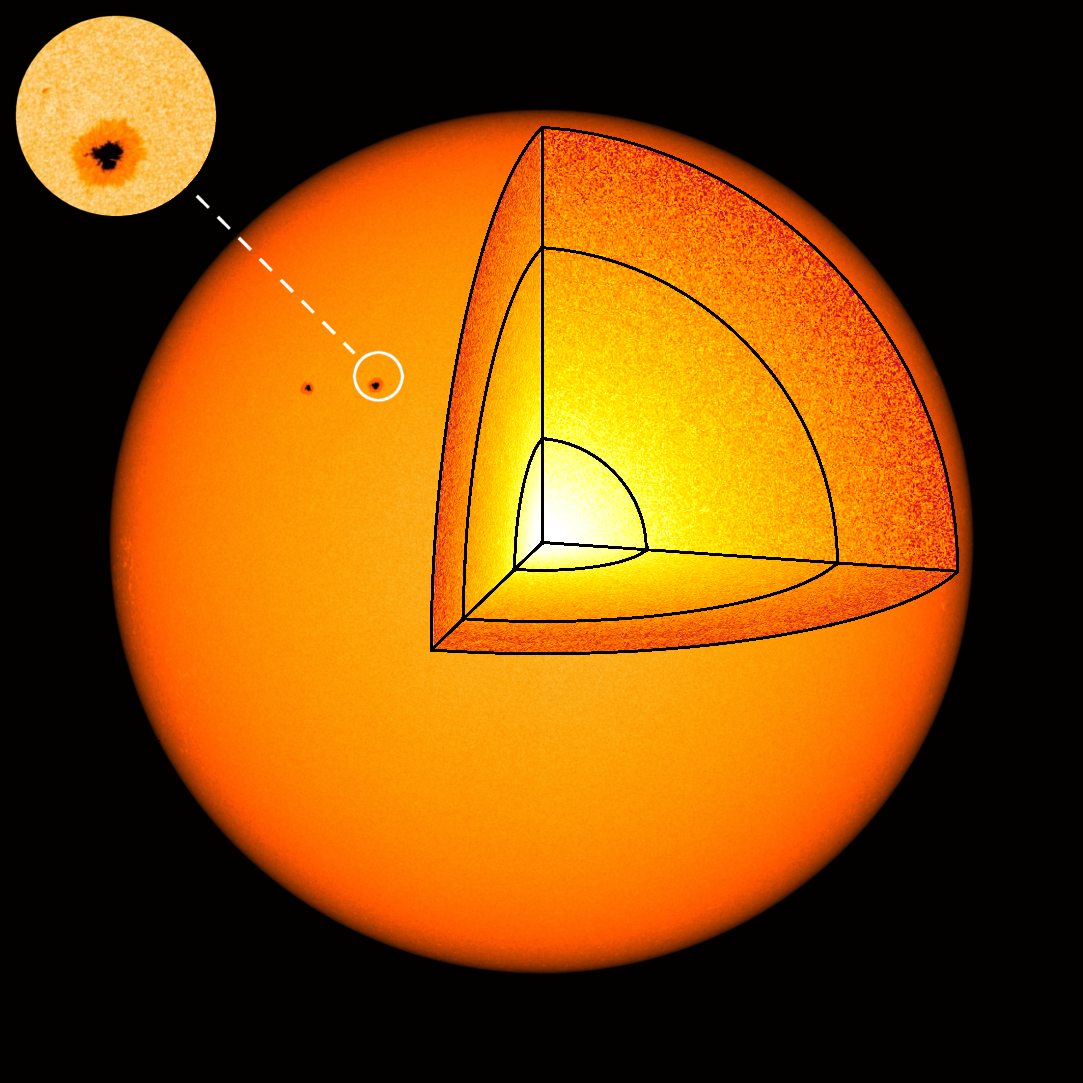
\includegraphics[width=0.6\textwidth]{images/own_figures/sun_interior_HMIIC.png}
	}{
		\caption{Image of the photosphere together with a schema of the solar interior structure. The inset shows the granular surface with a sunspot. The figure is based on a SDO/HMI continuum image from 20~March~2016, credit: NASA/SDO and the AIA, EVE and HMI science teams.}
		\label{fig:sun_interior_HMIIC}
	}
\end{figure}

%%% chromosphere + corona + CMEs
Above the photosphere at the base of the chromosphere the temperature declines to its solar minimum of \SI{3800}{\K} until it raises to \numrange{1}{3}~million~kelvins in the corona \citep{Billings1959}. Up to now it is not fully understood why the corona is so much hotter than the underlying chromosphere---this question is known as the coronal heating problem. The energy transfer mechanisms of choice are magnetic reconnections, wave heating and type~II spicules or a combination of these (cite?).

The chromosphere is a \SI{2000}{\km} thick region whose features (numerous spicules, filaments and prominences) can range far into the corona. They consist of by the solar magnetic field channeled chromospheric material, which is enveloped by a thin transition region where the temperature jumps up from ?\SIrange{20000}{35000}{\K} to coronal temperatures (cite?). Reconnection of magnetic field lines can result in the eruption of filaments into the corona and beyond, termed coronal mass ejections (CMEs) (see also Section~XX...). Details of chromospheric features are shown in \autoref{fig:sun_atmosphere}.

%%% coronal holes
The Sun's atmosphere is dominated by the varying small- and large-scale solar magnetic field configuration. There are regions where the magnetic field lines arc back to the surface and regions with open field lines. In the latter areas the coronal plasma can---guided by the field---escape into space. Thus these coronal areas are less dense, cooler and therefore appear darker in extreme ultraviolet (EUV) and are called coronal holes (more in Section~XX...). In \autoref{fig:sun_atmosphere} a coronal hole is located at the solar south pole.
\begin{figure}[htb]
	%\centering
	\fcapside[\FBwidth]{
		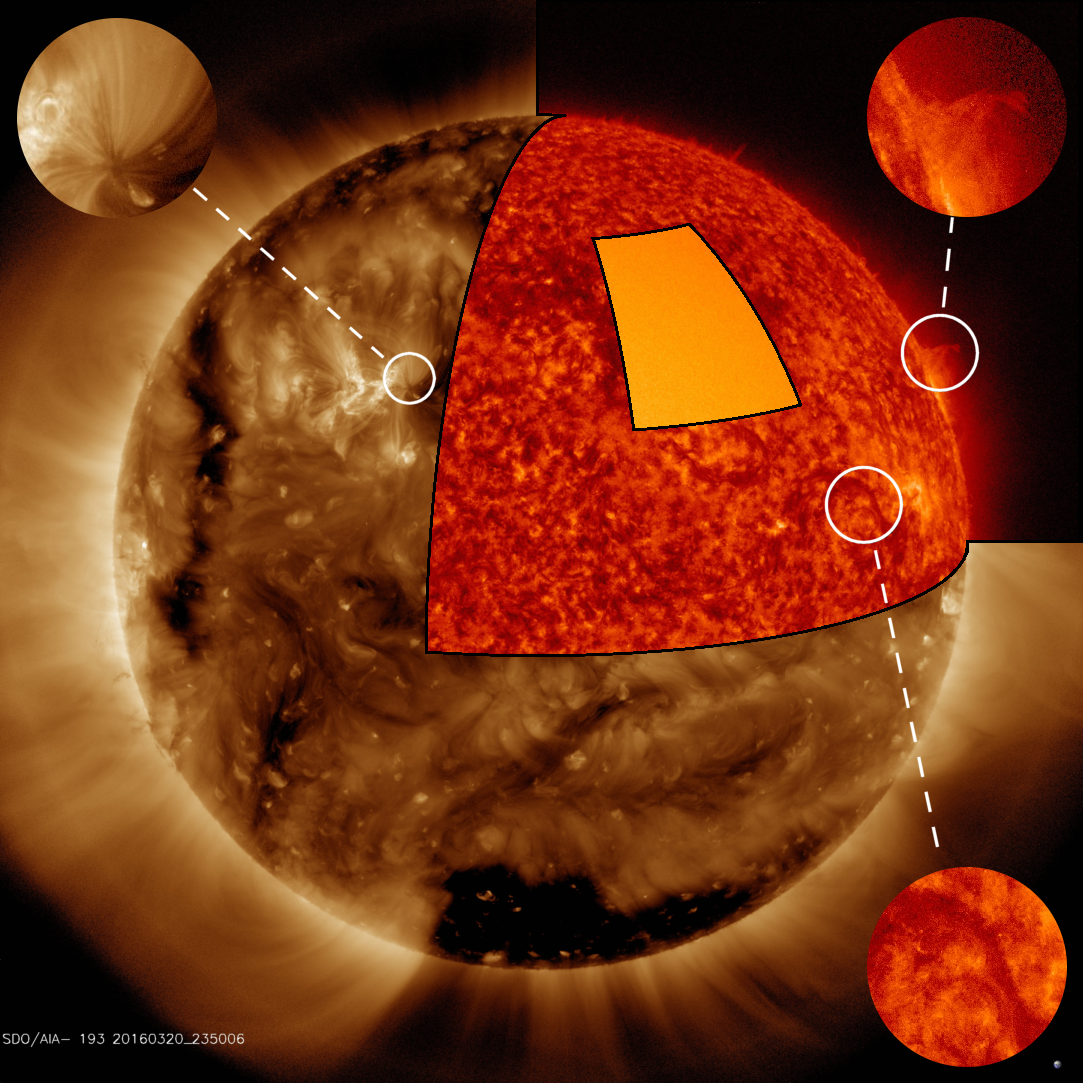
\includegraphics[width=0.6\textwidth]{images/own_figures/sun_atmosphere.png}
	}{
		\caption{Composite image of the solar atmosphere and some of its features. Corona, chromosphere and photosphere are seen in wavelengths of \SI{193}{\angstrom}, \SI{304}{\angstrom} and continu\-um. On the northern limb chromospheric spicules are visible. The enlargements on the right show a prominence and a filament. The dark region at the south pole is a coronal hole. The left inset shows details of the active region belonging to the sunspots in \autoref{fig:sun_interior_HMIIC}. The figure is based on SDO/AIA images from 20~March~2016, credit: NASA/SDO and the AIA, EVE and HMI science teams.}
		\label{fig:sun_atmosphere}
	}
\end{figure}

%%% corona
From Earth the faint corona and chromosphere can only be observed during eclipses, because of the brightness of the solar disk. There are three effects contributing to the visibility of the corona, photon scattering off free electrons and dust particles, and ion spectral emission lines (termed K-, F- and E"~corona).
% the so-called K-, F- and E"~corona (K kontinuierlich, F Fraunhofer, E emission).\\
% K-corona: photon scattering off free electrons --> coronagraphs\\
% F-corona: photon scattering off dust particles; contains Fraunhofer absorption lines; expands in ecliptic as zodiacal light --> coronagraphs\\
% E-corona: ion spectral emission lines; reveals coronal composition --> images\\
The image of a solar eclipse reveals the by the magnetic field shaped coronal plasma and features of the red chromosphere, pictured in \autoref{fig:Tse2008_500_mo1}.\\
\begin{figure}[htb]
	%\centering
	\fcapside[\FBwidth]{
		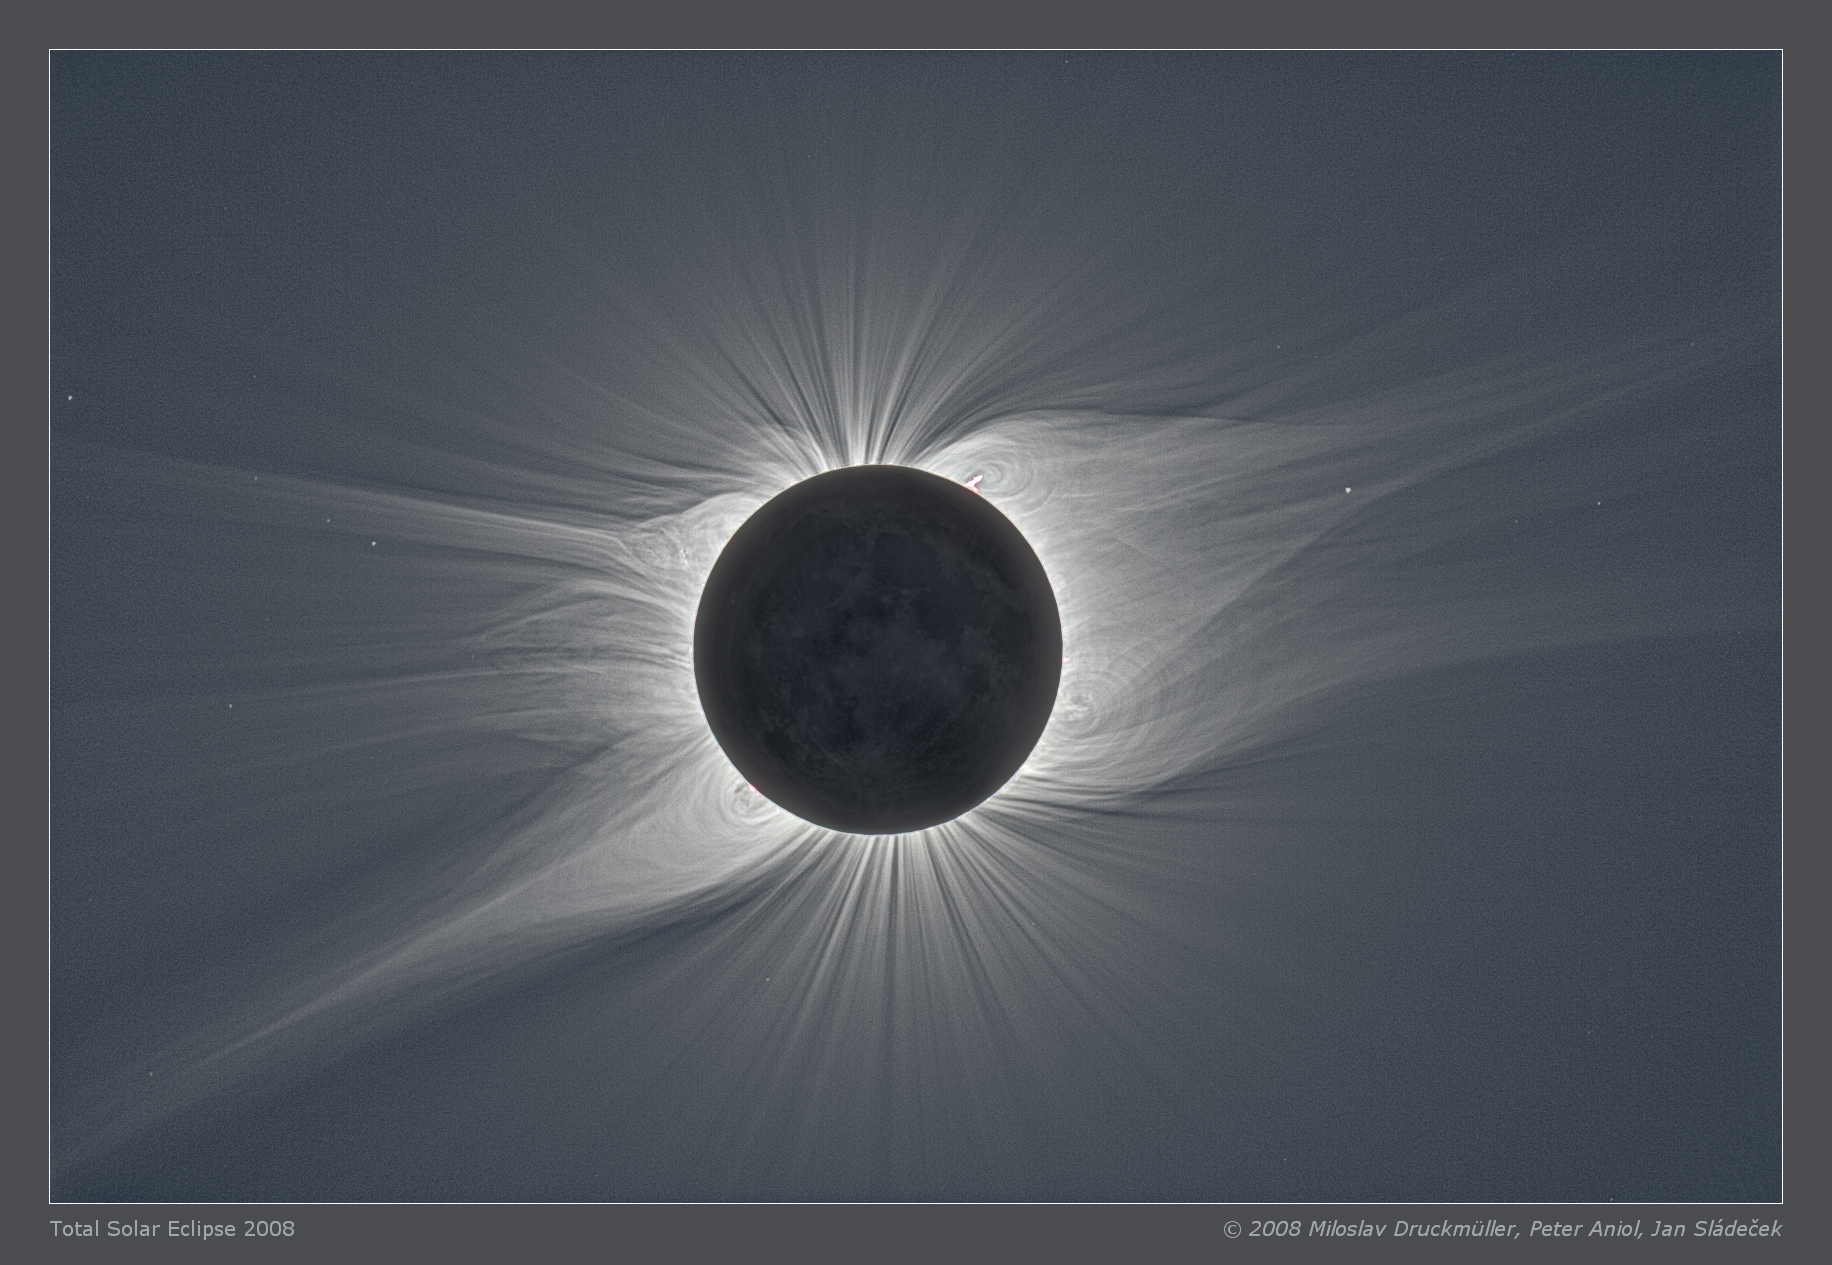
\includegraphics[width=0.6\textwidth]{images/Tse2008_500_mo1.png}
	}{
		\caption{Total solar eclipse image of the inner corona up to 5~solar radii. The picture was taken in Mongolia, 1~August~2008 and is processed from multiple images. Visible are the for a quiet Sun in cycle minimum typical magnetic field's dipole structure and the equatorial streamer belt. Credit: Miloslav Druckmüller, Peter Aniol, Jan Sládeček, 2008. get permission and preferred citation style... into acknowledgments? \url{http://www.zam.fme.vutbr.cz/~druck/Eclipse/}}
		\label{fig:Tse2008_500_mo1}
	}
\end{figure}
%figure source: http://www.zam.fme.vutbr.cz/~druck/Eclipse/Ecl2008m/Tse2008_500_mo1/Hr/Tse2008_500_mo1.png

%%% solar wind + heliosphere
Because of the high coronal temperatures, plasma escapes from the solar gravitational field \citep{Parker1958} with velocities of \SIrange{200}{800}{\km\per\s}. Its acceleration is linked to the coronal heating, but the exact location and process remain an open question (cite?). At a distance of a few solar radii (?4--20) the magnetic field becomes too weak to guide the coronal plasma. From this source surface the solar wind flows radially outward into space until it reaches the termination shock, spanning the heliosphere. Eventually it collides with the local interstellar medium, creating the heliopause. The heliosphere is expected to be a bubble of teardrop shape (and may be led by a bow shock), caused by the Sun's relative velocity of \SI{23}{\km\per\s} to the local interstellar medium \citep{Owens2013}. Measurements of the Voyager~1 and 2 spacecraft indicate their passage of the termination shock at about \SI{94}{\au} and \SI{84}{\au}, entering the heliosheath region \citep{Owens2013}. \citet{Gurnett2013} report that in 2012 Voyager~1 actually crossed the heliopause into interstellar space at a solar distance of \SI{121}{\au}. \autoref{fig:Owens2013_Heliosphere_screenshot} illustrates the heliosphere and its surrounding flow structure.\\
\begin{figure}[htb]
	%\centering
	\fcapside[\FBwidth]{
		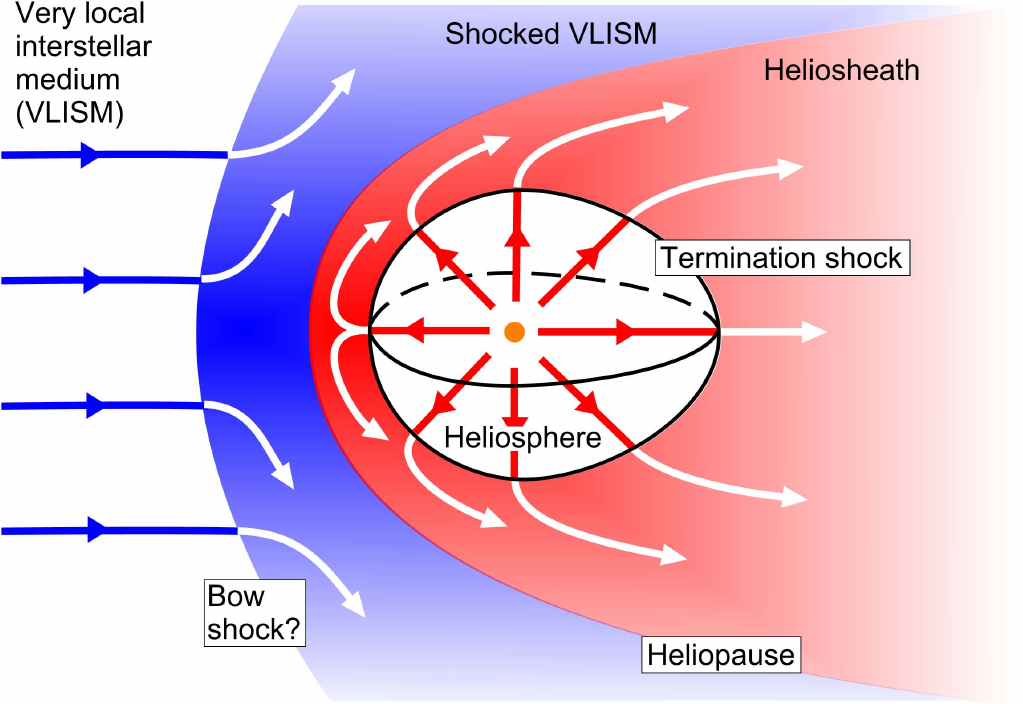
\includegraphics[width=0.6\textwidth]{images/Owens2013_Heliosphere_screenshot.png}
	}{
		\caption{Schema of the heliosphere and its surrounding flow structure. The heliosphere is formed by the interaction of the solar wind with the local interstellar medium at the heliopause. \citep[Fig.~9]{Owens2013} get permission...}
		\label{fig:Owens2013_Heliosphere_screenshot}
	}
\end{figure}

%%% solar wind influence + space weather
On its way outwards through the solar system the solar wind, carrying the solar magnetic field, interacts with the planets, their magnetic fields and other solar system bodies. These interactions have various effects, for instance disturbances in planetary magnetic fields with appearance of aurorae and enhanced radiation, atmospheric losses and stripping of cometary tails. Some of these effects can have disruptive consequences for humans and their technology. The topic of space weather effects is further addressed in \autoref{sec:space_weather}. The magnitude of these effects highly depend on spatial and temporal variations in the solar wind which are rooted in the dynamics of the solar magnetic field.\\

%%%%%%%%%%%%%%%%%%%%%%%%%%%%%
%\section{Stars/Beginning}
% introduction leading to stars; beginning from universe/big bang\\
% gravitational contraction of rotating nebula\\
% -> fusion burning; energy production\\
% In its core it fuses hydrogen to helium; 15.7~million~K; inner 25~\%\\
% energy transport -> radiation zone; up to 70~\%\\
% tachocline ~2~million~K\\
% energy transport by convection -> convection zone; up to surface\\
% convective granulation\\
% photoshere 4400--6600~K, effective black body temperature 5777~K; spectral class\\
% (herzsprung russell diagram)\\
% chromosphere... (solar atmosphere figure)\\
% transition region\\
%corona 1--3~million~K temperature (coronal heating problem)\\
% coronal holes: open magnetic field lines, solar wind\\
% heliosphere, shock with interstellar medium (ISM); Voyager\\

%%%%%%%%%%%%%%%%%%%%%%%%%%%%%
%big bang
%to formation of stars
%to ISM in our galaxy
%to formation of Sun
%Sun's inner structure (energy production and transport)
%its surface (radiation, spectral class)
%its outer structure (chromosphere, corona, solar wind, heliosphere)
%its heliosphere (termination shock with ISM, Voyager measurements)
%%%%%%%%%%%%%%%%%%%%%%%%%%%%%


\section{Solar dynamics}
\label{sec:solar_dynamics}

%%% differential rotation + solar magnetic field origin
The spin conservation of the contracting molecular cloud led to a rotation of the Sun with a current average period of about 25~days. The radial convective motion within the solar interior above the tachocline leads to a transport of momentum away from the rotation axis and therefore to a slower polar and faster equatorial rotation in the convection zone \citep{Miesch2005}. This differential rotation is visible on the surface and was first discovered from sunspot observations. %in 1630 https://en.wikipedia.org/wiki/Solar_rotation
With a rotation period of about 34~days the poles have a lag of almost 9~days (for further information on solar rotation see appendix \autoref{sec:solar_surface_differential_rotation}). The differential rotation in the solar interior can be inferred from helioseismological observations, as seen in \autoref{fig:Miesch2005_fig1a_interior_diff_rot}.\\
\begin{figure}[htb]
	\begin{floatrow}
		\ffigbox{	%[\FBwidth][]{
			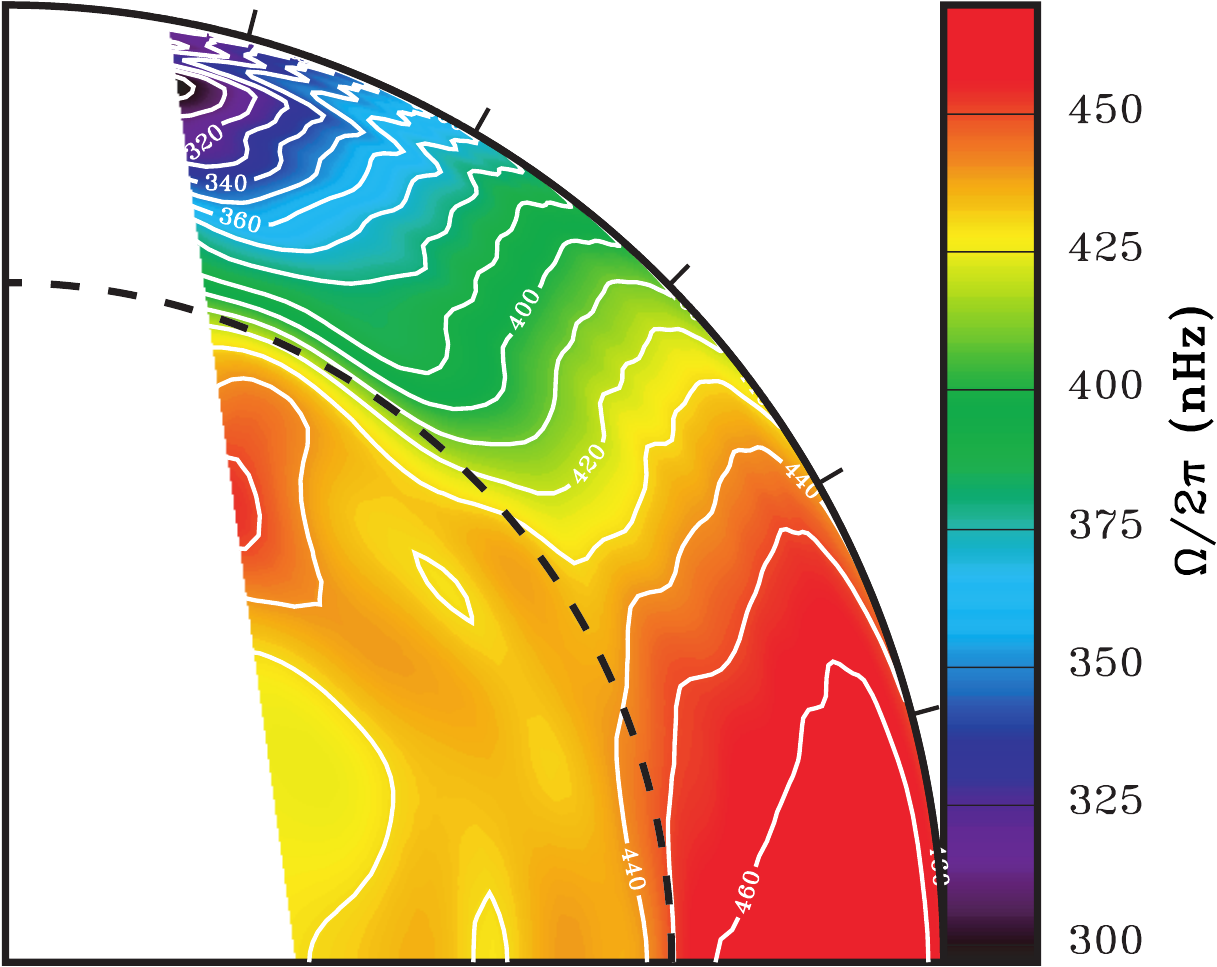
\includegraphics[width=0.5\textwidth]{images/Miesch2005_fig1a_interior_diff_rot.png}
		}{
			\caption{Angular rotation velocity in the solar interior. The radiation zone has a nearly solid rotation. Above the tachocline (dashed line) begins the differential rotation of the convection zone. The angular velocity is inferred from helioseismology via observations from the Michelson Doppler Imager (MDI) at the Solar and Heliospheric Observatory (SOHO) spacecraft. \citep[Fig.~3]{Thompson2003} get permission...}
			%(\citet[Fig.~1\,a]{Miesch2005}; based on \citet[Fig.~3]{Thompson2003})
			\label{fig:Miesch2005_fig1a_interior_diff_rot}
		}
		\ffigbox{
			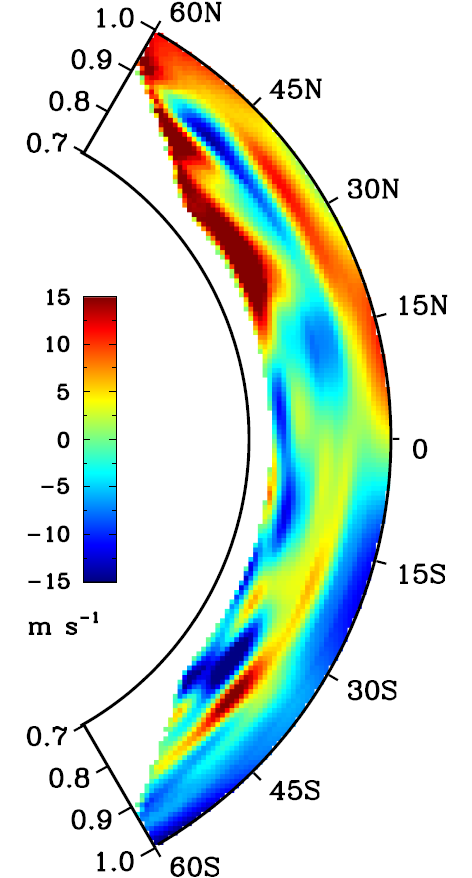
\includegraphics[width=0.28\textwidth]{images/Zhao2013_meridional_flow.png}
		}{
			\caption{Meridional flow velocity profile in part of the convection zone. Positive values are directed towards north. The velocity is inferred from helioseismology via observations from the Helioseismic Magnetic Imager (HMI) at the Solar Dynamics Observatory (SDO) spacecraft. \citep[Fig.~4\,a]{Zhao2013} get permission...}
			\label{fig:Zhao2013_meridional_flow}
		}
	\end{floatrow}
\end{figure}
%Angular velocity profile in the solar interior inferred from helioseismology (after Thompson et al., 2003). In panel (a), a 2D (latitude-radius) rotational inversion is shown based on the subtractive optimally localized averaging (SOLA) technique. All inversions are based on data from the Michelson Doppler Imager (MDI) instrument aboard the SOHO spacecraft, averaged over 144 days. Inversions become unreliable close to the rotation axis, represented by white areas in panel (a). Note also that global modes are only sensitive to the rotation component which is symmetric about the equator (courtesy M.J. Thompson \& J. Christensen-Dalsgaard).

The resulting large rotational shear at the tachocline generates toroidal magnetic flux ($\Omega$-effect?), which convectively raises to the surface forming sunspots. This solar dynamo is thought to create the major part of the solar magnetic field \citep{Miesch2005}.\\	%Miesch2005 p.~18 + p.~31

$\alpha\Omega$-dynamo\\

``Magnetic layer at the base of the convection zone; existence of a deep-seated layer in the Sun with strong toroidal magnetic fields; stronger magnetic fields can be stored for sufficiently long times in the stably stratified region below the convection zone; toroidal magnetic field has an intensity of the order B $\approx$ 1--10~T; the generation of strong toroidal magnetic fields near the bottom of the convection zone; '' \citep{Ossendrijver2003}\\

%%% convection cycle + solar surface magnetic field + solar cycle
Helioseismic measurements reveal that the large-scale convective flow is agglomerated into large convection cells with slow meridional flows of a few \si{\m\per\s}. A poleward subsurface flow and equatorward backflow beneath is detected within each hemisphere, see \autoref{fig:Zhao2013_meridional_flow}.\\

[The cells have a convection cycle of about 22~years (cite...). As the magnetic field is carried by the plasma, it emerges at the surface with the same periodicity.]\\

Within one period the surface magnetic field configuration changes from a dipole structure to a reversed dipole structure with opposite polarity, thus the transition time from one dipole state to the next lasts about 11~years.\\

In the transition phase toroidal magnetic flux emerges in belts above and below the solar equator manifesting as active regions, resulting in a multipolar structured magnetic field.\\

bipolar active regions are toroidal magnetic flux, which has emerged as a loop from below the photosphere (magnetic flux ropes). (see \autoref{fig:bipolar_region_HMIB_HMIIF})\\
\begin{figure}[htb]
	%\centering
	\fcapside[\FBwidth]{
		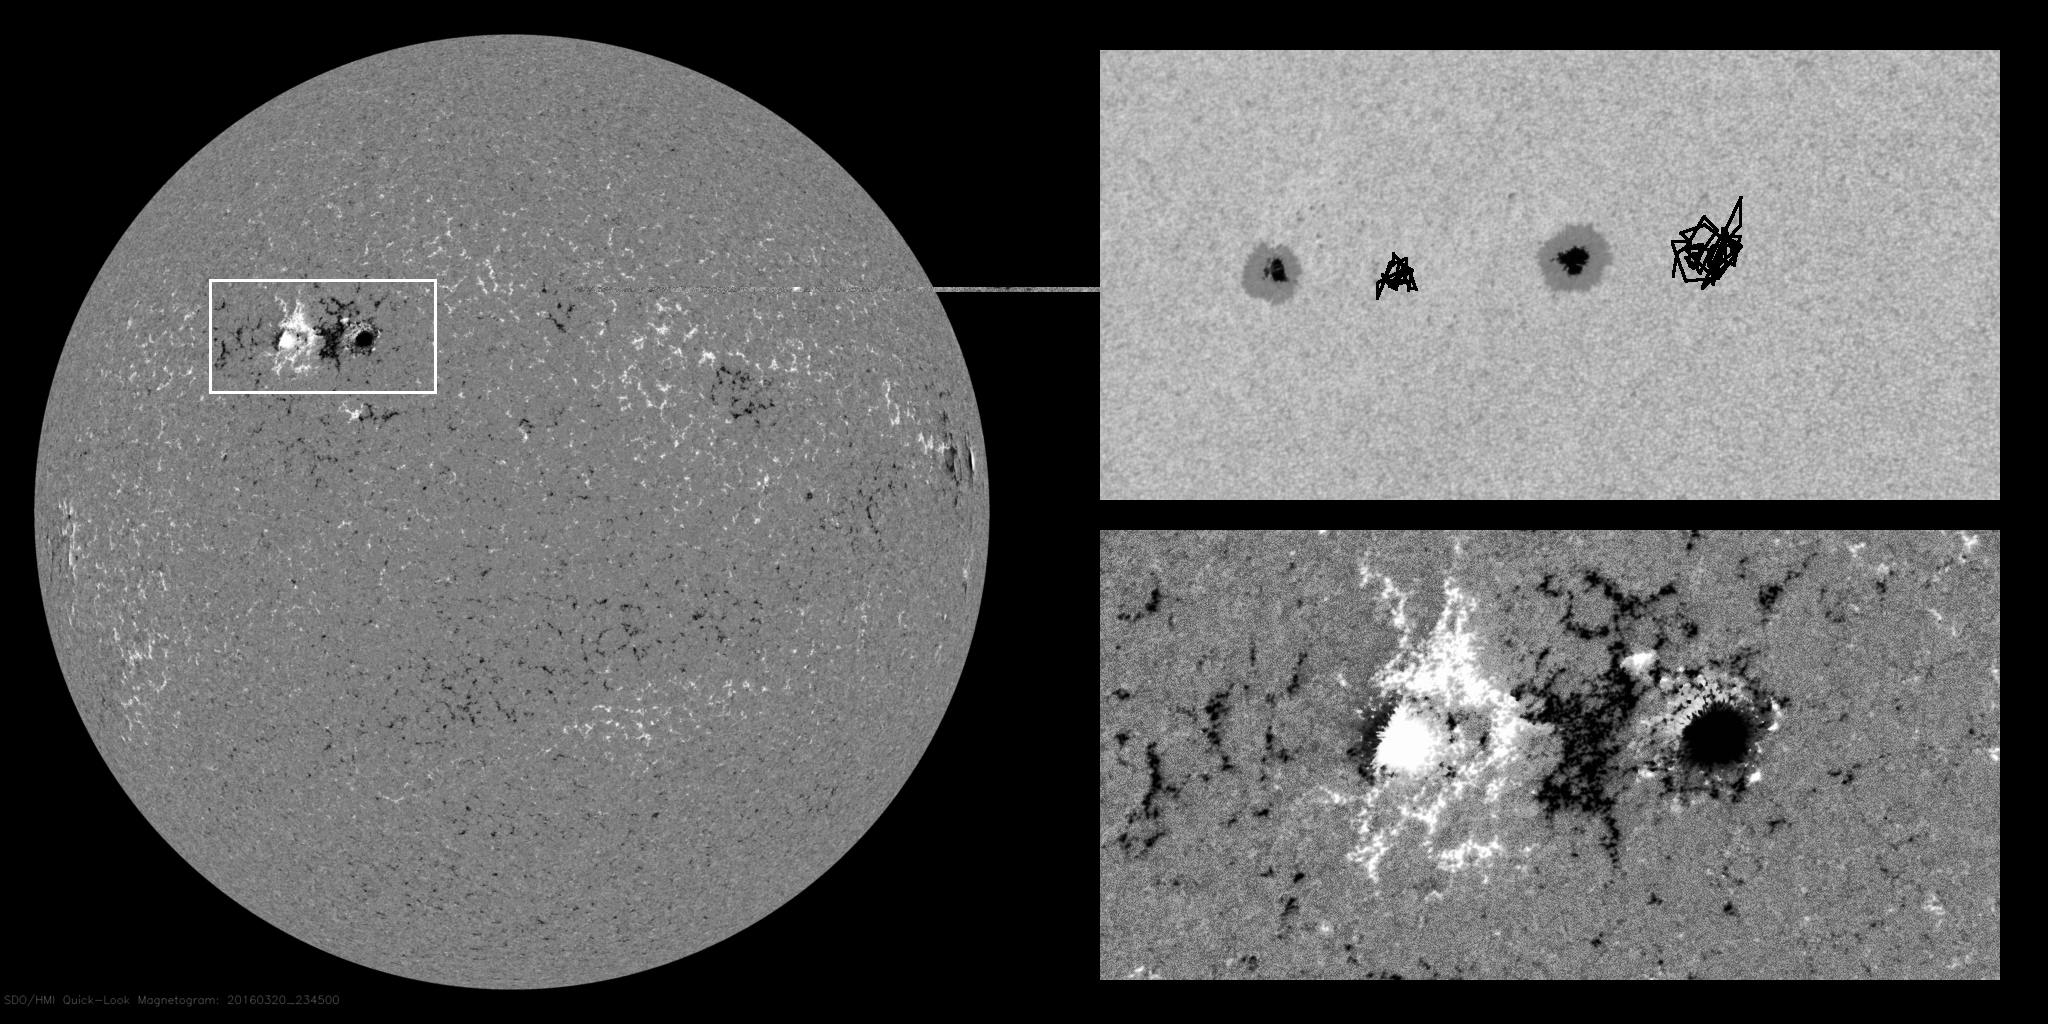
\includegraphics[width=0.6\textwidth]{images/own_figures/bipolar_region_HMIB_HMIIF.png}
	}{
		\caption{Continuum image of both sunspots from \autoref{fig:sun_interior_HMIIC}, magnetogram of the same region and of the whole solar disk. A magnetogram shows the polarity of the radial magnetic field component at the photosphere (black/white: xxward/xxward). The highly concentrated magnetic flux at the sunspots is clearly visible in the magnetogram as well as the extended bipolar magnetic field structure of the whole active region (black/white). The figure is based on SDO/HMI continuum and magnetogram images from 20~March~2016, credit: NASA/SDO and the AIA, EVE and HMI science teams. switch sides...}
		\label{fig:bipolar_region_HMIB_HMIIF}
	}
\end{figure}

poloidal field + diff. rot. => toroidal field ($\Omega$-effect) Miesch2005 p.~18 + p.~31\\
switching between states of strong poloidal and toroidal field\\

the solar dynamo: (toroidal to poloidal field)\\
- turbulent plasma motions from convective flows generate disorganized magnetic fields\\
- differential shear at tachocline amplifies fields to strong coherent toroidal flux ($\Omega$-effect); magnetic layer located at the base of the convection zone\\
- stronger flux ropes raise to surface (buoyantly)\\
- Coriolis force twists them systematically, stronger at higher latitudes\\
- twisted tubes emerge on the surface as bipolar active regions\\
- amplification of mean fields by fluctuating motions ($\alpha$-effect) and turbulent diffusion create large-scale poloidal field\\


%%% sunspots
Since regions of strong magnetic flux are visible as sunspots on the photosphere, they were known well before the common era by chinese and greek scholars. %greek sunspot observation: http://adsabs.harvard.edu/abs/2007JBAA..117..346V
Systematic sunspot observations exist since 1610, shortly after the invention of the telescope (cite?). In 1843 Schwabe discovered the 11-year periodicity in the sunspot occurence (cite?). To record solar cycles in 1848 Wolf (et al?) introduced the sunspot number (SSN) and cycle number (with the zeroth occuring in 1749) (cite?), see \autoref{fig:ROB_ssn_wolfmms}.\\
\begin{figure}[htb]
	%\centering
	\fcapside[\FBwidth]{
		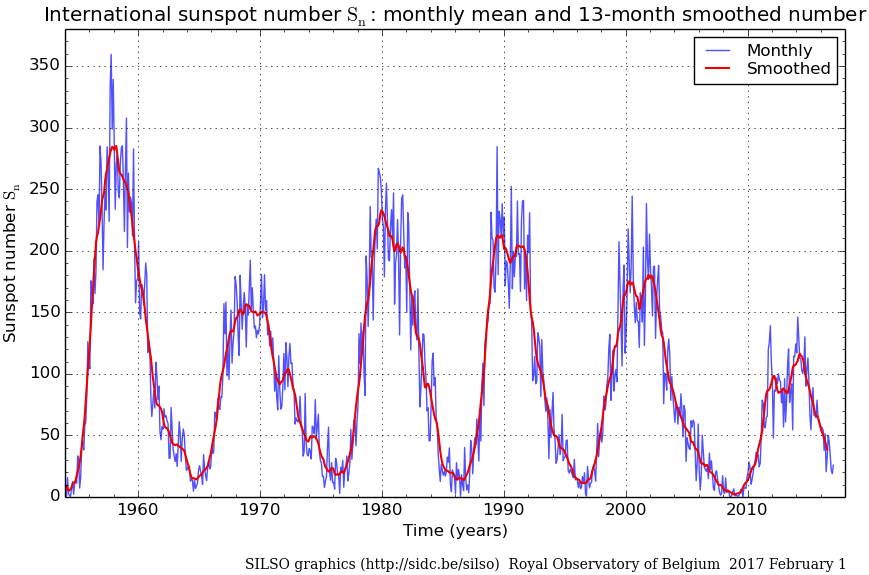
\includegraphics[width=0.6\textwidth]{images/ROB_ssn_wolfmms.png}
	}{
		\caption{Monthly mean sunspot number (blue) and 13-month smoothed monthly sunspot number (red) since 1954. Credit: SILSO data/image, Royal Observatory of Belgium, Brussels, \mbox{2017-02-01}. get permission... Update this figure before printing!!!}
		\label{fig:ROB_ssn_wolfmms}
	}
\end{figure}
%image from:	http://sidc.be/silso/
The large variations in cycle length ?(9--14~years) and intensity ?(\SIrange{0}{350}{S_n}) make it difficult to predict the course of the next solar cycle (cite...).\\
long-time variations like the Maunder minimum... see Hathaway2015\\

%butterfly
Observations of the surface radial magnetic field show the appearance of bipolar magnetic flux at belts of about \SI{+-20}{\degree} latitude at the beginning of a cycle and a shift towards lower latitudes at the end of a cycle (magnetogram figure of sunspot?). Thus the plot of surface magnetic field over latitude and time reveals a butterfly pattern. The emerging flux (its polarity alternates with each cycle) is carried by the slow meridional surface flow poleward, resulting in the polar field switch, see \autoref{fig:Hathaway_magbfly}. The ordered dipole structure in solar cycle minimum leads to open polar field regions with large coronal holes and a closed equatorial field belt/streamer belt (clearly visible in \autoref{fig:Tse2008_500_mo1}).\\
\begin{figure}[htb]
	\centering
	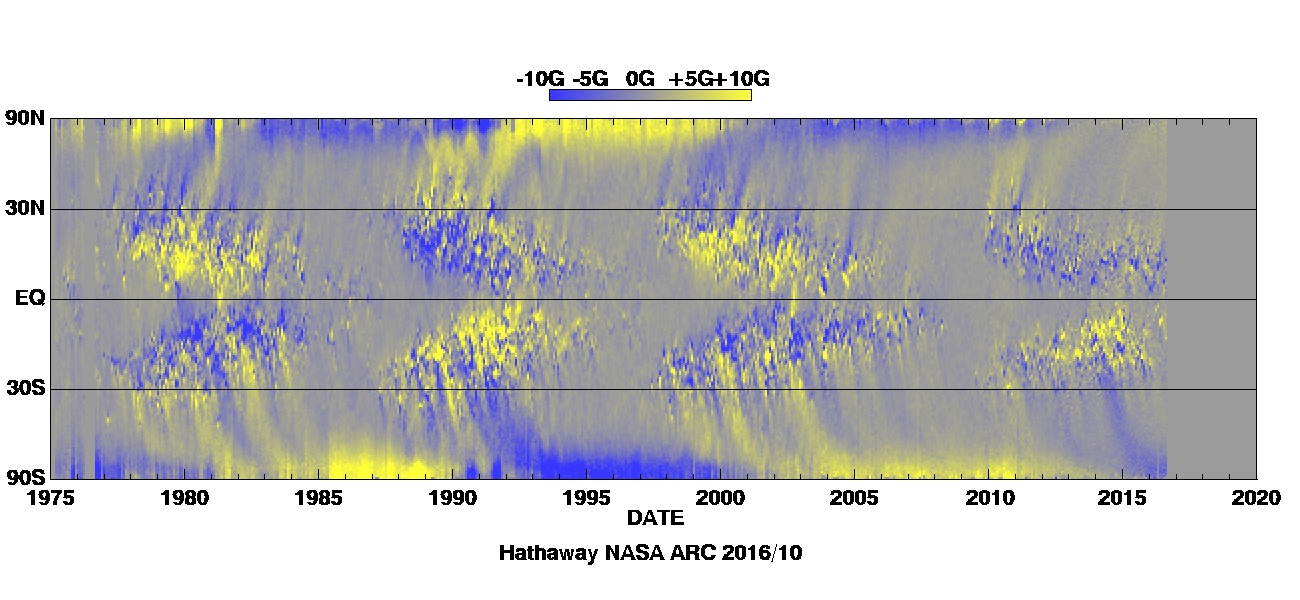
\includegraphics[width=\textwidth]{images/Hathaway_magbfly_201610.jpg}
	\caption{This magnetic butterfly diagram maps the synoptic radial magnetic field on the solar surface. Yellow represents an outward directed magnetic field (positive), blue inward (negative). The data is obtained from instruments on Kitt~Peak National Observatory and from the MDI at the SOHO spacecraft. Credit: David~Hathaway, NASA Marshall Space Flight Center; see also \citet[Fig.~17]{Hathaway2015}. Update this figure before printing! get permission...}
	\label{fig:Hathaway_magbfly}
\end{figure}
%figure source:	http://solarscience.msfc.nasa.gov/images/magbfly.jpg

sunspot butterfly pattern \citep{Maunder1904}\\

sunspots NE active regions; active regions forming streamer belt?\\

The magnetic field geometry during cycle maximum is more complex, due to the in mid-latitudes emerging flux, which is related to the then stronger toroidal component of the solar magnetic field.\\

HMF with figures DQCS + Parker spiral\\

This leads to the chaotic appearance of closed field lines even at higher latitudes/poles and coronal holes covering equatorial regions. tbm\\

sw in minimum: streamer belt and polar HSSs\\

fast solar wind emerges from CHs\\

slow from closed field streamers\\

This is confirmed by the Ulysses spacecraft, which measured the solar wind speed in a polar orbit covering more than one solar cycle (\autoref{fig:McComas2008_Ulysses_orbit}).\\
\begin{figure}[htb]
	\centering
	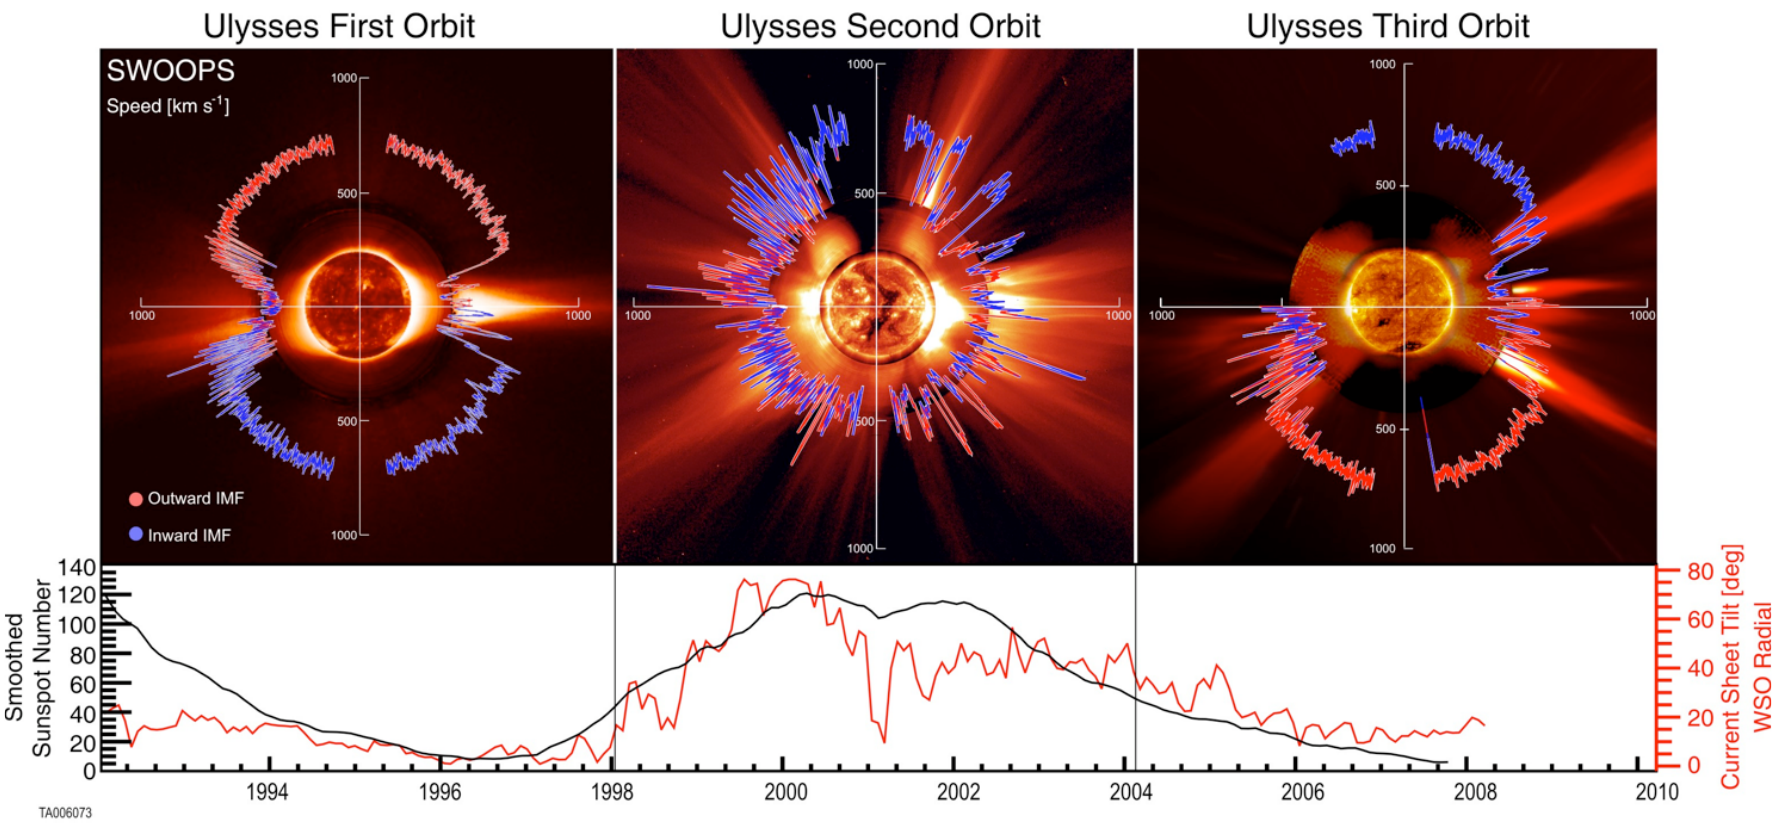
\includegraphics[width=\textwidth]{images/McComas2008_Ulysses_orbit_.png}
	\caption{Solar wind velocity and magnetic field polarity over latitude during low and high solar activity for the three orbits of the Ulysses spacecraft. The SSN and CS tilt angle are plotted as well. \citep[Fig.~1]{McComas2008}. ask for high res. image and permission...}
	\label{fig:McComas2008_Ulysses_orbit}
\end{figure}
%figure source: http://onlinelibrary.wiley.com/doi/10.1029/2003GL017136/full
%McComas2008: (a–c) Polar plots of the solar wind speed, colored by IMF polarity for Ulysses' three polar orbits colored to indicate measured magnetic polarity. In each, the earliest times are on the left (nine o'clock position) and progress around counterclockwise. (d) Contemporaneous values for the smoothed sunspot number (black) and heliospheric current sheet tilt (red), lined up to match Figures 1a–1c. In Figures 1a–1c, the solar wind speed is plotted over characteristic solar images for solar minimum for cycle 22 (8/17/96), solar maximum for cycle 23 (12/07/00), and solar minimum for cycle 23 (03/28/06). From the center out, we blend images from the Solar and Heliospheric Observatory (SOHO) Extreme ultraviolet Imaging Telescope (Fe XII at 1950 nm), the Mauna Loa K coronameter (700–950 nm), and the SOHO C2 white light coronagraph.

%++dynamics and magnetic field++\\
%rotating nebula to solar rotation\\
%rotation + convective motion -> differential rotation (first discovered by sunspot observations; helioseismology -> inner rotation, tachocline)\\
% meridional flow -> 22 year cycle || convective cells\\
% 22y convection cycle + magnetic field -> 11ys solar cycle (magnetic field activity cycle, polarity change, sunspot number)\\
keywords:\\
SSN -> magnetic surface activity (butterfly diagram) => poloidal/toroidal field -> min/max polar CHs (quiet/active Sun figure) -> HMF (quiet B-field figure) -> quiet HMF Parker spiral (figure) -> solar wind -> slow/fast sw pattern (Ulysses figure))\\

solar wind plasma composition and proberties -> visible solar wind structures (coronagraph image; with CME and streamer) -> stream interface (figure) -> in situ measurements (example in situ CIR/HSS plot)\\

stream interfaces (figure and link to previous CIR plot) -> HCS/HPS\\

CMEs (link to previous coronagraph image; in situ CME/MC plot; CME schema figure?)\\

differential rotation/shear at tachocline -> B-field\\
meridional flow -> solar cycle period\\
dipole structure, open and closed field lines\\
polar coronal holes\\
streamer/equatorial streamer belt\\
solar wind\\

open field lines (coronal holes) -> HSSs\\
equatorial ballerina model -> CIRs (figure?)\\

%%% reconnections + CMEs
The solar differential rotation wraps the magnetic field lines, accumulating tension, leading eventually to relief with a magnetic reconfiguration by field line reconnections.\\
--> release of much energy --> flares, CMEs\\


solar wind's impact on Earth\\

the rotation axis is tilted from the normal of the ecliptic by $i_\odot = 7.25$\textdegree{} \citep{USNO2015} (refer to or put into appendix??).\\ %USNO2015 C3

%%%%%%%%%%%%%%%%%%%%%%%%%%%%%%%%%


\section{Solar wind}
\label{sec:solar_wind}

see Kivelson1995, p14+91\\
first observed at solar eclipses?, before? deduced by Parker from theory/Carrington from geomagnetic storms?\\

discovered via eclipses?\\
see eclipse photo from Druckmüller \autoref{fig:Tse2008_500_mo1}\\

in 1958 Parker predicted/postulated the solar wind \citep{Parker1958}\\
expanding isothermal atmosphere (solar wind model)\\
continuous supersonic radial outflow of plasma\\
-> also Parker spiral of HMF (see \autoref{fig:Owens2013_PFSS_Sectors_screenshot})


\section{Heliospheric magnetic field}	%better: interplanetary magnetic field??
%\label{sec:heliospheric_magnetic_field}

reviews: \citet{Balogh2009} (for heliosheath), \citet{Owens2013}\\

Winterhalter1994 The heliospheric plasma sheet:\\
"the narrow heliospheric current sheet (ca. 3000--10000 km thick), together with the heliospheric plasma sheet in which it is embedded. The heliospheric plasma sheet region is identified by a significantly enhanced plasma beta caused by density enhancements and diminished magnetic field strength and is about 20 to 30 times the thickness of the current sheet."\\
heliospheric current sheet (HCS)\\
heliospheric plasma sheet (HPS)\\
ballerina model... (search figure...)\\

%Cranmer2005:
%?insert their figure 1
Photosphere: magnetic bright points (MBP) 1--2~kG\\ %Cranmer2005
their convective motion result in wavelike fluctuations of the thin tubes\\
low chromosphere: thin flux tubes expand laterally and merge to a homogeneous network field\\
below the chromosphere-corona transition region: the network magnetic field expands laterally and merges again to a large-scale canopy (image)\\

[above the Alfv\'en critical point---where the wind speed equals the local Alfv\'en speed at about 10~$R_\odot$---both the inward and outward modes are advected (advect: convect horizontally) outward with the wind\\
superradially expanding magnetic flux tube\\
\citep{Cranmer2005}]\\
see also paper citations...\\

analytical solar magnetic field model for solar minimum conditions \citep{Banaszkiewicz1998}\\
dipole plus quadrupole plus current sheet (DQCS) solar magnetic field model\\
The DQCS model with its quadrupole part having a direct link from the solar equator to infinity along the equatorial plane and current sheet. (see \autoref{fig:Banaszkiewicz1998_DQCS_model_raw}) \citep{Banaszkiewicz1998}\\
compare with field geometry from eclipse \autoref{fig:Tse2008_500_mo1}...\\
\begin{figure}[htb]
	\begin{floatrow}
		\ffigbox{
			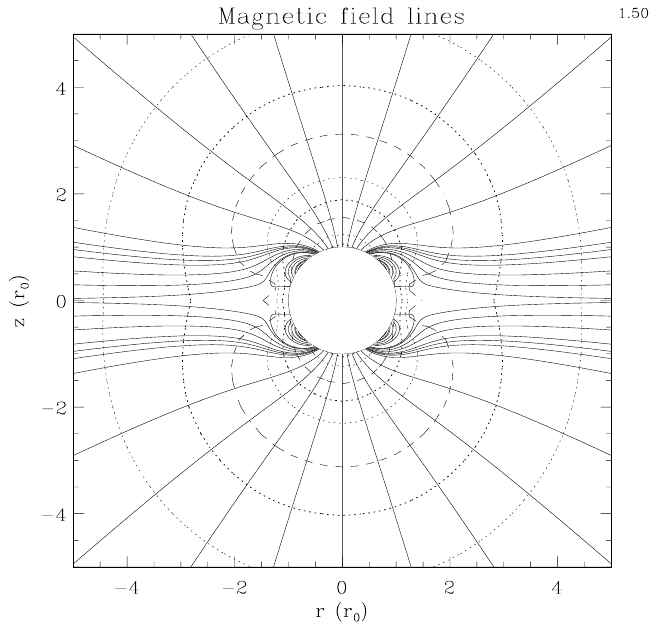
\includegraphics[width=0.45\textwidth]{images/Banaszkiewicz1998_DQCS_model_raw.png}
		}{
			\caption{Solar magnetic field geometry from the DQCS model with field lines (solid) and constant field strength surfaces (dashed). The quadrupole part allows equatorial outflows along the current sheet. \citep[Fig.~3]{Banaszkiewicz1998} get permission...}
			\label{fig:Banaszkiewicz1998_DQCS_model_raw}
		}
		\ffigbox{
			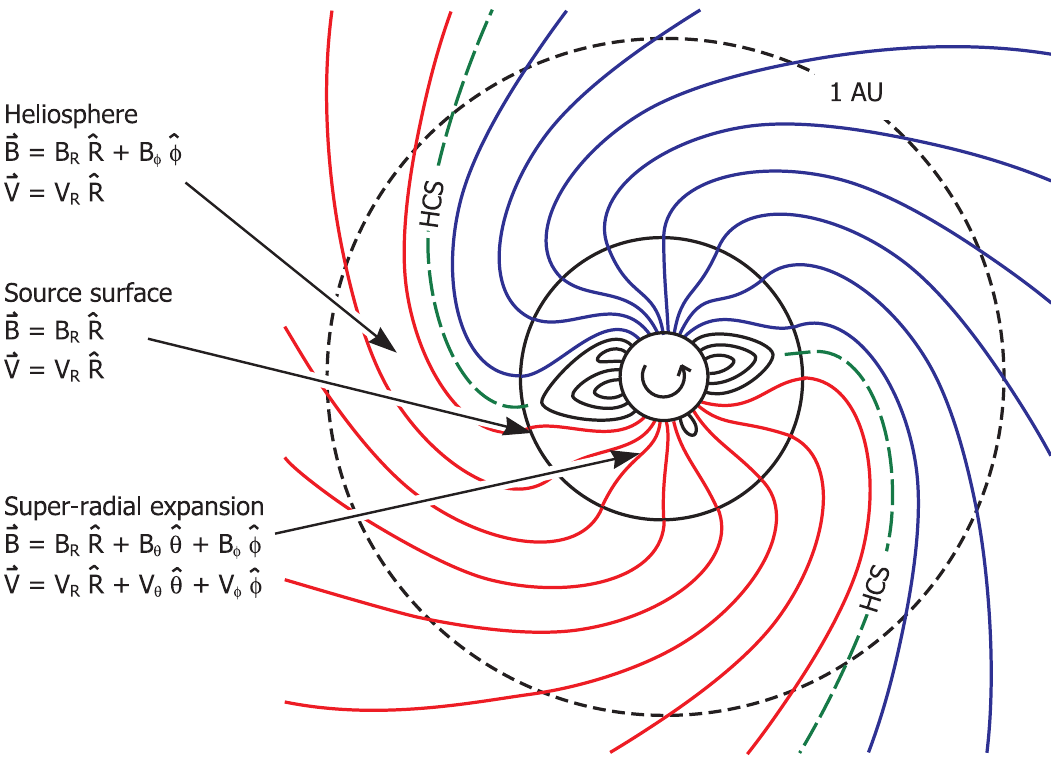
\includegraphics[width=\Xhsize]{images/Owens2013_PFSS_Sectors_screenshot.png}
		}{
			\caption{Illustration of the solar magnetic field Parker spiral formation by rotation of the solar wind source surface. Between solar wind flows of opposite magnetic field polarity a heliospheric current sheet (HCS) forms. (\citet[Fig.~1]{Owens2013}, adapted from \citet[Fig.~1]{Schatten1969}) get permission...}
			\label{fig:Owens2013_PFSS_Sectors_screenshot}
		}
	\end{floatrow}
\end{figure}

Parker spiral, source surface and HCS, see \autoref{fig:Owens2013_PFSS_Sectors_screenshot}\\
%A sketch of the steady-state solar magnetic field in the ecliptic plane. Close to the Sun, in a spatial region approximately bounding the solar corona, the magnetic field dominates the plasma flow and undergoes significant non-radial (or super-radial) expansion with height. At the source surface, typically taken to be a few solar radii, the pressure-driven expansion of the solar wind dominates and both the field and flow both become purely radial. In the heliosphere, rotation of the HMF footpoints within a radial solar wind flow generates an azimuthal component of the HMF, leading to a archimedean spiral geometry. Regions of opposite HMF polarity, shown as red and blue lines, are separated by the heliospheric current sheet (HCS), shown as the green dashed line. Image adapted from Schatten et al. (1969).

MHD simulations based on Voyager~1 and 2 measurements within the heliosheath indicate the formation of magnetic bubbles (reconnected sector regions) at the sector boundary caused by the compression before the heliopause, flowing away to the heliosheath tail \citep{Opher2011}.\\
%Opher2011: Is the Magnetic Field in the Heliosheath Laminar or a Turbulent Sea of Bubbles?


\section{Solar wind properties and structures}

list event/structure types\\
solar wind structures source regions: sunspots/active regions, coronal holes, filaments\\

sw density considerations, see presi S³\\

\subsection{Solar wind plasma}
\label{sec:solar_wind_plasma}

Plasma in general (properties (H/He/metal composition; see paper...), Plasma-beta, etc.)\\
	solar wind properties, slow/fast wind, MHD waves (Alfv\'en waves)\\

special events/configurations, which can appear (CIRs, HCS/HPS, etc.)
HSS, sector boundaries, CIRs, CMEs\\


\subsection{Slow solar wind}

regions with closed lines\\
trapped plasma, slow solar wind from streamers\\


\subsection{High speed streams}

regions with open lines\\
coronal holes as sources of fast sw\\

sw plot of HSS with CIR to refer to\\

\citet{Schwenn1983}: ``During the Skylab era in 1973/74 we learned that these high speed streams emerge from coronal holes (Hundhausen, 1977 and references therein).''\\


\subsection{Stream interaction regions}

Streams of fast wind catch slow wind\\
-> compressions, shocks, deflections\\

Corotating interaction regions (CIRs)\\
Stream interaction regions (SIRs)\\

formation of stream interface and stream deflection, see \autoref{fig:Owens2013_CIR_2panel_screenshot}\\
%A sketch of a stream interaction region. Left: Looking down on the ecliptic plane. Magnetic field lines within fast (slow) wind, shown in red (blue), become aligned with the stream interface by the reverse (forward) wave. Right: a view from Earth. The magnetic axis, M, and therefore the wind speed belts, are inclined to the rotation axis, R. The point in the heliosphere at which fast wind is able to catch up to the slow wind ahead of it is the stream interface (SI), which forms a spiral front in the heliosphere, shown as the black-outlined curved surface. In the frame of reference of the SI, both fast and slow wind flow toward the SI. Fast (slow) wind, shown by the red (blue) arrow, is slowed (accelerated) and deflected along the SI in the direction counter to (along) solar rotation. Right panel adapted from Pizzo (1991).
\begin{figure}[htb]
	%\centering
	\fcapside[\FBwidth]{
		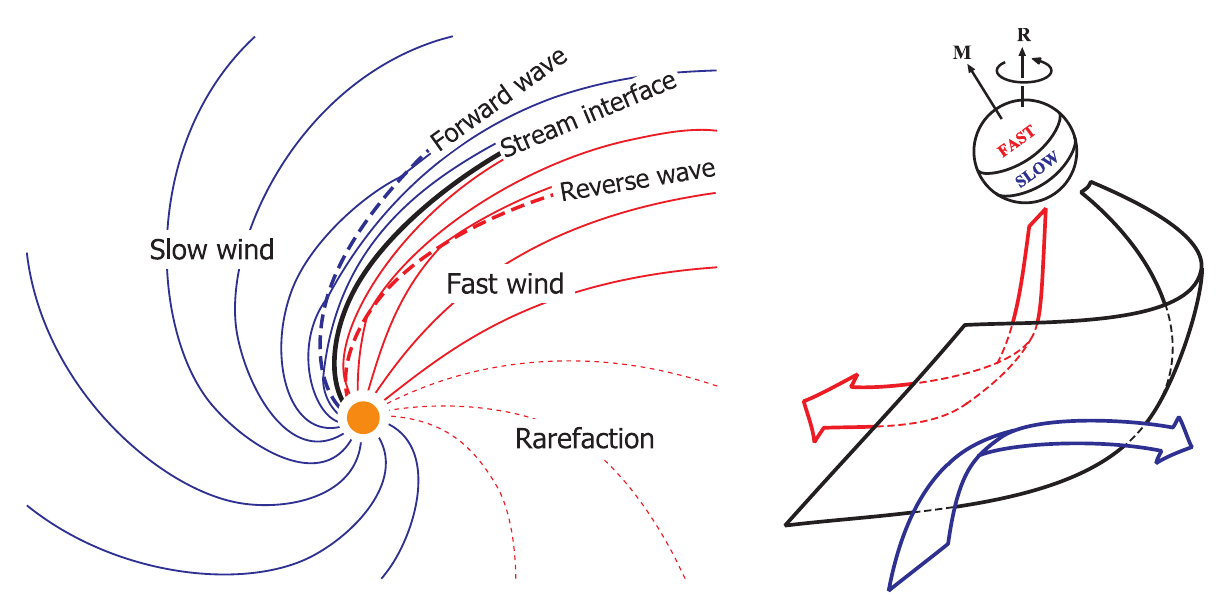
\includegraphics[width=0.6\textwidth]{images/Owens2013_CIR_2panel_screenshot.png}
	}{
		\caption{Schema of the formation of a stream interface (left) and deflection of streams (right), both generated from interactions between slow and fast solar wind. (\citet[Fig.~7]{Owens2013}; right panel adapted from \citet[Fig.~2]{Pizzo1991}) get permission...}
		\label{fig:Owens2013_CIR_2panel_screenshot}
	}
\end{figure}
refer to sw figure of CIR\\


\subsection{HCS / HPS}

from sector boundaries (ballerina skirt)\\


\subsection{Coronal mass ejections}
\label{sec:coronal_mass_ejections}

Coronal mass ejections (CMEs) (discovery (Carrington), definition (Hundthausen?), models, GCS (conception of 3-dim CME shape --> enables Earth arrival time forecast from modeled direction and velocity))\\

active regions:\\
sunspots, magnetic reconnections, flares, post-eruptive arcades\\

coronagraph figure of CME (COR2 image, SECCHI/STEREO)\\
in situ solar wind figure of same CME (recent one from 2016)\\

CME-plasma properties\\
+ flares and SEPs often accompany CMEs\\

\subsubsection{Magnetic clouds}
magnetic cloud (MC); refer to in situ plot\\
See BS magnetic cloud model in analyses methods chapter
MVA...\\


\section{Space weather}
\label{sec:space_weather}

Solar wind influences the Earth's magnetosphere and can disturb sensitive technical systems\\
understanding its properties helps with prediction of events\\

influences on human infrastructure/technical systems\\

various space weather effects, for instance disturbances in magnetic fields, aurorae, episodes of enhanced radiation, atmospheric losses and stripping of cometary tails. figures of these effects?\\

reference to \citet{Bothmer2007}, maybe images\\

\subsection{Solar influence on Earth}
\label{sec:solar_influence_on_earth}

Carrington made first connection between terrestrial magnetic field and solar flares. correct?\\

%see Bartels1962:
there are several types of solar-terrestrial relations, \citet{Bartels1962} listed:\\	%Zuordnung solarer Beobachtungen zu terrestrischen\\
a) irregular flare and CME effects (Carrington)\\
b) 11"~year solar cycle effects\\
c) 27"~day solar rotation effects\\
d) daily effects (x-ray and light)\\

seasonal effects from Earth orbital distance, inclination (solar rotation axis angle) and Earth tilt (see \autoref{fig:sun-earth_seasonal_geometry_draft})\\
\begin{figure}[htb]
	\centering
	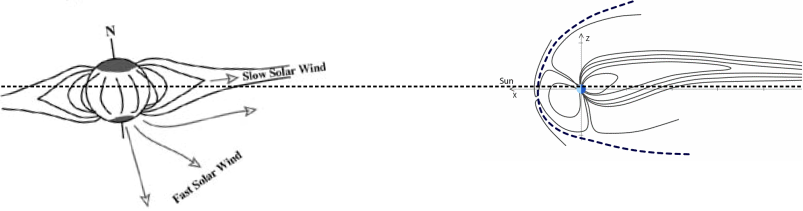
\includegraphics[width=\textwidth]{images/own_figures/sun-earth_seasonal_geometry_draft.png}
	\caption{Sun-Earth geometry in the plane orthogonal to the ecliptic (not to scale); Solar magnetic field-magnetosphere geometry. Seasonal effects are: solar tilt, Earth distance and Earth tilt}
	\label{fig:sun-earth_seasonal_geometry_draft}
\end{figure}

solar wind and its species\\
solar radiation\\
solar energetic particles (SEPs)\\
gravitation\\

magnetosphere\\
ionosphere?\\
aurorae\\
geomagnetic storms (several days, from CMEs)\\
substorms (few hours, from CIRs??)\\

for humans and their technology important effects: enhanced radiation, geomagnetic storms\\
lovely, disruptive, dangerous consequences <-- read in VBbook\\

at Earth the solar wind total energy flux ($1.45~\text{mW/m}^2$) is only about one millionth of the solar radiation flux (see \citet[p.~153]{Schwenn1990})\\

"The principal users affected by geomagnetic storms are the electrical power grid, spacecraft operations, users of radio signals that reflect off of or pass through the ionosphere, and observers of the aurora." NOAA cite\\

\subsection{Magnetosphere}
\label{sec:magnetosphere}

shape formed by dynamic pressure..., similar to heliosphere in ISM...\\

bow shock, magnetotail, magnetosheath, magnetopause\\
add ecliptic and terrestrial tilt angle; with plasmoid?\\
see \autoref{fig:heliosphere_image002}\\
\begin{figure}[htb]
	%\centering
	\fcapside[\FBwidth]{
		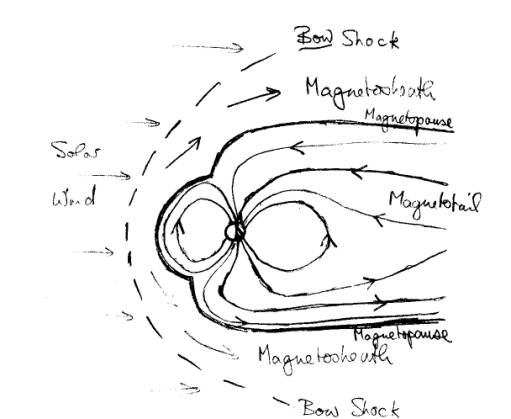
\includegraphics[width=0.5\textwidth]{images/heliosphere_image002.jpg}
	}{
		\caption{temp figure ``The cavity is called the magnetosphere. It has a relatively well-defined outer boundary, the magnetopause.''}
		\label{fig:heliosphere_image002}
	}
\end{figure}

turbulence with sw (KH or RT instabilities), see \autoref{sec:solar_wind_magnetosphere_coupling}\\

Earth magnetic field strength at a height of 36\,000~km (geostationary): ~100~nT\\
Earth magnetic field strength at the surface - equator: ~30\,000~nT - poles: ~60\,000~nT (cite?)\\

magnetopause = current layer??\\

two extreme cases of Bz orientation: parallel/antiparallel\\
compression/reconnection (see \autoref{fig:Bothmer1998book_p116_fig4_8_sw})\\
\begin{figure}[htb]
	%\centering
	\fcapside[\FBwidth]{
		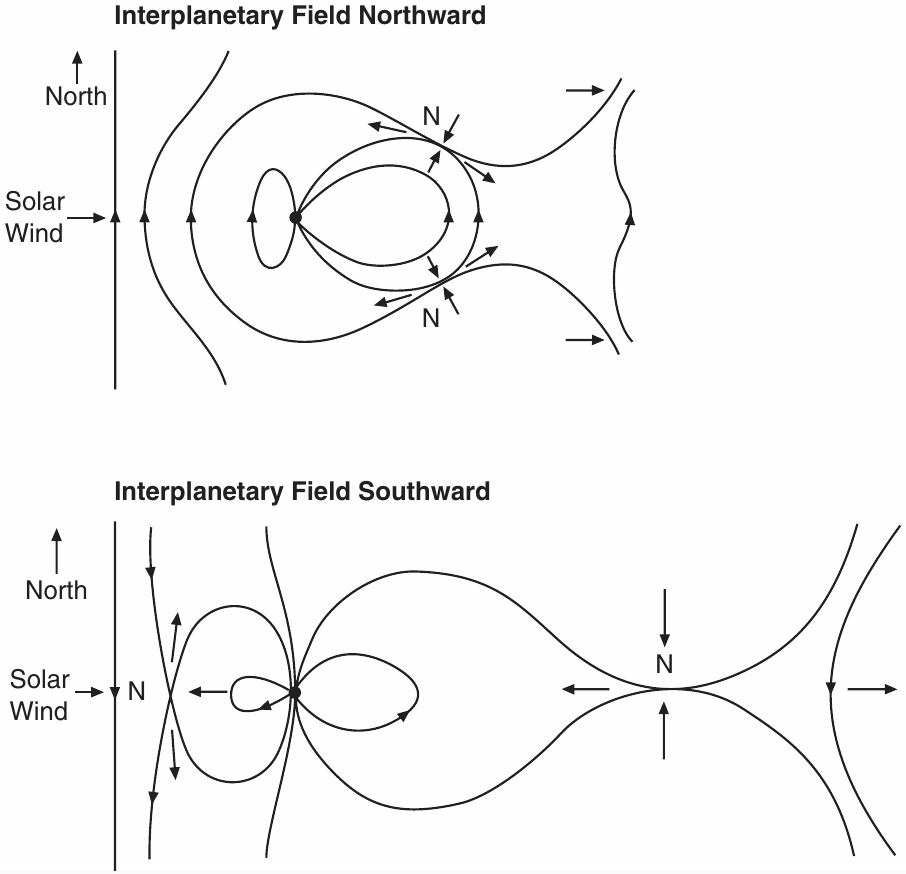
\includegraphics[width=0.5\textwidth]{images/Bothmer1998book_p116_fig4_8_sw.png}
	}{
		\caption{reconnection and compression depending on the interplanetary magnetic field orientation; figure~4.8 from \citet[p.~116]{Bothmer1998}, adapted from Dungey1961, 1963. accelerated flows are arrowed; N points are X points...}
		\label{fig:Bothmer1998book_p116_fig4_8_sw}
	}
\end{figure}

standoff distance:	\citep[p.~112]{Bothmer2007}
\begin{align}
	d = \frac{107.4}{1 R_\text{E}} (N V^2)^{-1/6}
\end{align}

Even in ``ancient'' times (when?) a correlation between solar particles and disturbances in the magnetosphere were known of (Bartels1962).\\

magnetosphere variations due to solar wind\\
magnetosphere protects from radiation (maybe from solar wind stripping atmosphere away?)\\

effects: aurorae, ...\\

ring current systems\\

definition of:\\
magnetic storm...\\
substorm...\\

subsection Ionosphere?\\
its variations due to solar radiation (day/night cycle and flares)\\
ionosphere -> TEC -> GNSS error\\


\subsection{Geomagnetic indices}
\label{sec:geomagnetic_indices}
Geomagnetic observatories are distributed widely over the globe, measuring the local magnetic field at their position. Several sets of stations, covering specific regions, are defined to monitor the state of different parts of the magnetospheric system. Magnetic measurements from these sets define several geomagnetic indices. The International Association of Geomagnetism and Aeronomy (IAGA)  supports the following global geomagnetic indices which are serviced by the International Service of Geomagnetic Indices (ISGI)\footnote{ISGI website: \url{http://isgi.unistra.fr/}}:
The $aa$~index is designed to represent the amplitude of the global geomagnetic activity, normalized to a geomagnetic latitude of \SI{+-50}{\degree}. The $am$~index characterizes the global geomagnetic activity. The \Kp{}~index is designed to measure geomagnetic disturbances from solar particle radiation [reword...]. The \Kp~index is described in more detail in \autoref{sec:kp_index}. The $Dst$~index monitors the intensity of the magnetospheric ring current. The $PC$~index monitors the polar cap magnetic activity -- it approximates the amount of energy which entered the magnetosphere through solar wind coupling. The $AE$~index and its relatives $AU$, $AL$ and $AO$ measure the magnetic effects of the northern auroral electrojet.
The first three listed indices (\textit{aa}, \textit{am} and \Kp{}) are calculated from different sets of local 3"~hourly $K$~indices, which measure the local magnetic disturbances at the observatories. There exist several more indices that are based on some of those listed above.\\

[for \Kp{}, $AA$ and $Dst$ read Section 7.4 in book \citet{Bothmer2007}...\\
$Dst$ (read book Jursa1985 p. 4-31)]\\


\subsection{Solar wind--magnetosphere coupling}
\label{sec:solar_wind_magnetosphere_coupling}

E"~field:	%VBth p124
\begin{align}
	\textbf{E}_\text{IMF?} = -\textbf{V} \times \textbf{B}_\text{IMF}
\end{align}
...derive from Lorentz force\\
(Because of high plasma conductivity the E"~field is not existent.)\\

Axford1964 viscous interaction (of turbulent nature, KH/RT instabilities, KH instabilities at the flanks of the magnetosphere) is a viable source of drag force/solar storm energy input into magnetosphere\\

Otto\&Nykyri1982 KH instabilities/vortices force magnetic reconnection even at northern IMF and are able to account for observed mass flux\\

\citet{Newell2007} and \citet{Newell2008}: coupling consists of merging and viscous part (reconnection and turbulence)\\
merging part: rate magnetic flux is opened at the magnetopause\\
viscous part: reconnection due to Kelvin-Helmholtz instabilies at the boundary\\

Merkin2013 MHD simulation of velocity shear at magnetosphere boundary with northern IMF; KH instabilities; double-vortex sheet structure\\


\chapter{Data}
\label{chap:data}

%COFI -- chapter outline and flow integration\\


\section{Instruments}
%\label{sec:instruments}

For analyzing the solar wind and related effects on the Sun there are remote instruments (solar imager and coronagraphs) and in situ instruments (magnetometer and plasma detector).\\
Here the basic principles of the latter are described, because the analyses performed in this thesis are based on in situ solar wind measurements.\\

\subsection{Magnetometer}
%\label{sec:magnetometer}

Spacecraft nowadays carry two different magnetometer types, one for measuring the magnetic field direction and its strength and the other for observing the magnetic flux and detecting waves.\\

A flux gate magnetometer consists of two coils around a core---one coil with alternating current, wich is compared with the induced current signal from the other. Without external magnetic field both patterns match. The core is easier magnetized in direction of an existing external magnetic field, in which case the patterns differ. It measures...\\
In a search coil magnetometer one coil is placed around a core; measures plasma waves - where?\\

Because these magnetometer types are directional, they often are placed in two sets of triaxial configurations, attached on booms to minimize the influence of the spacecraft's own magnetic field.\\
L-> which is generated by surface charges?/electrons?/ionization?/the instruments?\\
%https://en.wikipedia.org/wiki/Spacecraft_magnetometer


\subsection{Plasma detector}
%\label{sec:plasma_detector}

several spectrometers with different energy ranges\\

isotope spectrometer - isotopic abundances of SEPs\\
ionic charge analyzer - charge state of SEPs\\
sw ion mass spectrometer - \\
sw ion composition spectrometer - \\
radio burst tracker\\


A plasma detector measures the ion energy frequency distribution, which consists basically only of protons and alphas in solar wind (see \autoref{fig:ion_energy_spectrum_plot}). see also \autoref{sec:solar_wind_plasma}
\\
\begin{figure}[htb]
	%\centering
	\fcapside[\FBwidth]{
		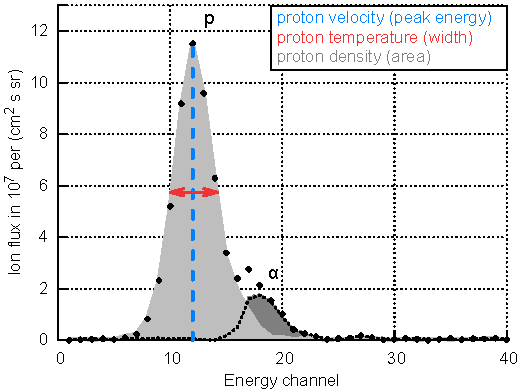
\includegraphics[width=0.5\textwidth]{images/gnuplots/ion_energy_spectrum_plot.pdf}
	}{
		\caption{Example of an ion energy spectrum with synthetic data. Here proton and helium (alpha) peaks are distinguishable...}
		\label{fig:ion_energy_spectrum_plot}
	}
\end{figure}
%figure adapted from source: http://www.goembel.biz/sun.html

From the energy spectrum the velocity, density and temperature can be derived.\\

The bulk velocity is derived from the distribution's average energy.\\
The number density is the area of the distribution.\\
The temperature scales with the distribution's width.\\

% source: ftp://spdf.gsfc.nasa.gov/pub/data/ulysses/plasma/swoops/ion/swoops_ion_users_guide_update_20030214.txt
% ``Plasma parameters are calculated by numerical integration of velocity-weighted
% ion distributions over an E/q range chosen to include the thermal proton and
% alpha-particle populations. Under extremely hot conditions, there can
% sometimes be some overlap between these populations. Additionally, during
% periods when the solar wind temperature is exceptionally low the experiment can
% not properly measure the temperature. Care has been taken to estimate the
% instrument background from channels that do not contain data, and the effects
% of background have been removed from the integration. The velocity space 
% resolution of the experiment is better in the energy dimension than in the
% angular dimensions.''


\section{Data sources}
%\label{sec:}

Spacecraft / data sets\\

Positions:\\
Earth:\\
	imager, magnetosphere\\
L1 - Lagrangian point:\\
	ACE (siehe auch space weather spacecraft Liste)\\
	Wind etc. (OMNI)\\
inner heliosphere:\\
	Helios~1 \& 2\\
outer heliosphere:\\
	Voyager~1 and 2\\
	Ulysses\\

also RT-data sources?\\


\subsection{Sunspot number}
%\label{sec:sunspot_number}

SSN history\\
add SSN figure of history incl. Maunder minimum?\\

SIDC/SILSO...\\
WDC-SILSO -- World Data Center-Sunspot Index and Long-term Solar Observations\\
%https://de.wikipedia.org/wiki/Sonnenfleck#Geschichte


\subsection{\Kp{}~index}
\label{sec:kp_index}
Julius~Bartels introduced the \textit{K}~index in 1938 and designed it to measure the intensity of geomagnetic disturbances \citep{Bartels1939}. Its name originates from 'Kennziffer' -- the german word for characteristic digit. The \textit{K}~index is a measure for the maximal variation of the surface magnetic field, observed in a magnetogram within 3"~hour intervals. Its scale in the range 0--9 is a quasi-logarithmic representation of the actual magnetic field strength's variations.

The Planetary \textit{K}~index (\Kp{}) is a planetary geomagnetic disturbance index, introduced by Bartels in 1949 at the Institute for Geophysics, University of Göttingen \citep{Bartels1949}. \Kp{} is the weighted average of 13 \textit{Ks}~indices, which are the standardized versions of the local \textit{K} indices measured at 13 observatories. These contributing observatories are located around \SI{+-50}{\degree} geomagnetic latitude and their distribution is biased towards Europe (see \autoref{fig:Kp_map}).
\begin{figure}[htb]
	%\centering
	\fcapside[\FBwidth]{
		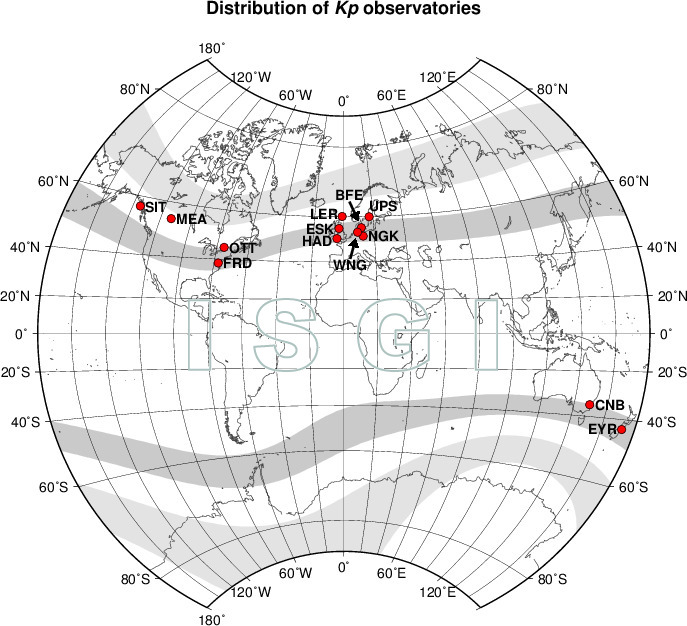
\includegraphics[width=0.6\textwidth]{images/Kp_map.jpg}
	}{
		\caption{Distribution of the 13 \Kp{} observatories. Credit: International Service of Geomagnetic Indices (ISGI), 2013. look into cc license...}
		\label{fig:Kp_map}
	}
\end{figure}
%\url{http://isgi.unistra.fr/indices_kp.php}

To benefit from its higher precision, its scale, in the range 0--9 as well, is further divided into thirds, represented by the suffixes '$+$', 'o' and '$-$' (e.g., 3o, $3+$, $4-$, 4o). The \Kp{}~indices are often visualized in musical diagrams, where they are stacked into periods of 27~days to enable the detection of recurrent activities, as seen in \autoref{fig:musi1612}.
\begin{figure}[htb]
	\centering
	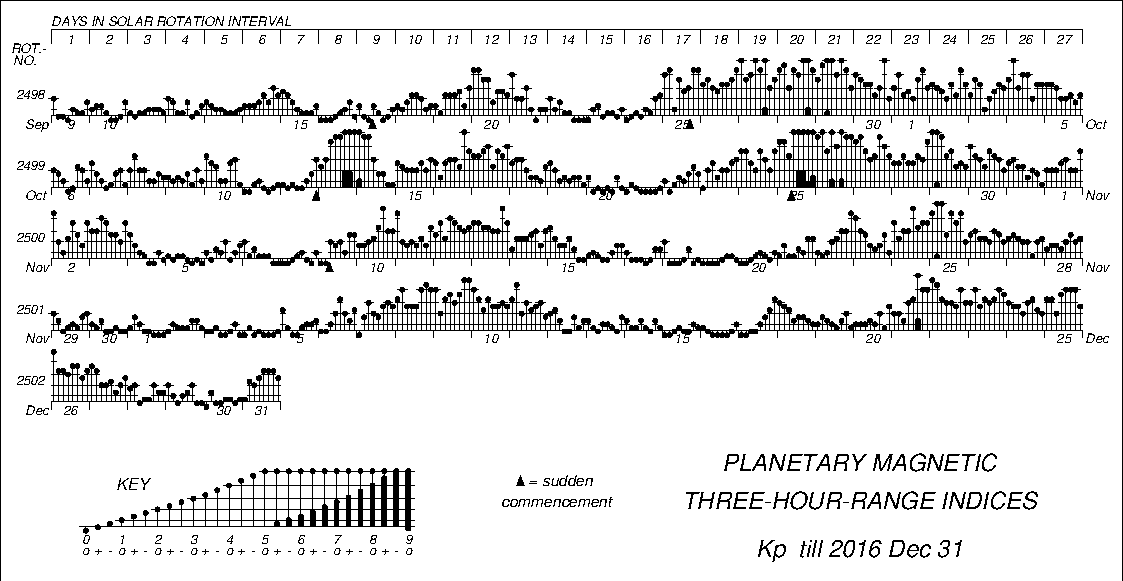
\includegraphics[width=\textwidth]{images/musi1612.pdf}
	\caption{Bartels musical \Kp{} diagram for the time period from September until end of December 2016. Two sudden commencements with following geomagnetic storms, having a maximal \Kp{} of $6+$, can be seen in October. Credit: GFZ~Potsdam, 2017. look into cc license...}
	\label{fig:musi1612}
\end{figure}
%ftp://ftp.gfz-potsdam.de/pub/home/obs/kp-ap/music/

The \Kp{}~intex can be converted to the 3"~hour equivalent $ap$~index, which represents the magnetic field strength at a surface position of about \SI{50}{\degree} dipole latitude. The conversion is done via a table defined by Bartels, in which the value of the \textit{ap}~index is scaled in units of \SI{2}{nT} (see \autoref{tab:kp_to_ap_table}).
\begin{table}
	\caption{Defined table for the conversion from the \Kp~index to the equivalent \textit{ap}~index, which represents the magnetic field strength in units of \SI{2}{nT}.}
	\label{tab:kp_to_ap_table}
	\centering
	\begin{tabular}{lssssssssssssss}
		\Kp	&0o	&0+	&1-	&1o	&1+	&2-	&2o	&2+	&3-	&3o	&3+	&4-	&4o	&4+\\
		\textit{ap}	&0	&2	&3	&4	&5	&6	&7	&9	&12	&15	&18	&22	&27	&32\\
		\hline
		\Kp	&5-	&5o	&5+	&6-	&6o	&6+	&7-	&7o	&7+	&8-	&8o	&8+	&9-	&9o\\
		\textit{ap}	&39	&48	&56	&67	&80	&94	&111	&132	&154	&179	&207	&236	&300	&400
	\end{tabular}
\end{table}
There are further geomagnetic indices which are derived from the \Kp{}~index. They include $Ap$, the daily $ap$ average, $Cp$, the daily $ap$ sum mapped via a defined table to the range \numrange{0}{2.5} and $C9$, a mapping of $Cp$ via a defined table to the range \numrange{0}{9}. The definitions of Q"~days (quiet days) and D"~days (disturbed days) are also obtained from the \Kp{}~index.

The International Association of Geomagnetism and Aeronomy (IAGA) adopted the \Kp{}~index in 1954. The \Kp{}~index was maintained in Göttingen until January 1997 -- now the German Research Centre for Geosciences (GFZ) in Potsdam supplies the \Kp{}~index and thereof derived indices. The GFZ provides historical and quicklook data of the indices via their website\footnote{GFZ website for geomagnetic indices: \url{http://www.gfz-potsdam.de/de/kp-index/} (existent in 2017-10-29)}. The data was extended backwards and is available from 1932 onwards.\\

further uses of the \Kp~index:\\
The NOAA G"~Scale for geomagnetic storms (G~1 to G~5) is based on the \Kp~index\footnote{NOAA Space Weather Scales website: \url{http://www.swpc.noaa.gov/noaa-scales-explanation} (existent in 2017-10-29)}.\\
GNSS error, auroral boundary positions\\

``It is designed to measure solar particle radiation by its magnetic effects.``\\

% acknowledgments:\\
% The results presented in this thesis rely on the \Kp{}~index, calculated and made available by the German Research Centre for Geosciences in Potsdam from data collected at magnetic observatories. We thank the involved national institutes, the INTERMAGNET network and ISGI (isgi.unistra.fr).\\


\subsection{OMNI data set}
\label{sec:omni_data_set}

a data set merged from different sources\\
The OMNI data \citep{King2005} were obtained from the GSFC/SPDF OMNIWeb interface.\\

from spacecraft located near the Lagrange point L1 upstream of Earth\\
time-shifted to the bow shock of the magnetosphere\\

OMNI2 H0 MRG1HR (1963-201308)
Cite from CDAweb: Hourly near-Earth solar wind magnetic field and plasma data, energetic proton fluxes (>~1 to >~60~MeV), and geomagnetic and solar activity indices.

NASA, Goddard Space Flight Center (GSFC), Space Physics Data Facility (SPDF): \url{http://spdf.gsfc.nasa.gov/}\\	%exintent in 2016-08-18
- Coordinated Data Analysis Web (CDAWeb): \url{http://cdaweb.gsfc.nasa.gov/}\\	%exintent in 2016-08-18
- OMNIWeb Plus: \url{http://omniweb.gsfc.nasa.gov/}\\	%exintent in 2016-08-18
%OMNIWeb Data Documentation: http://omniweb.gsfc.nasa.gov/html/ow_data.html


OMNI spacecraft data coverage (see also talk 2014-02-18)\\
see \autoref{fig:omni_data_coverage_1963-2013_plot}
\begin{figure}[htb]
	%\centering
	\fcapside[\FBwidth]{
		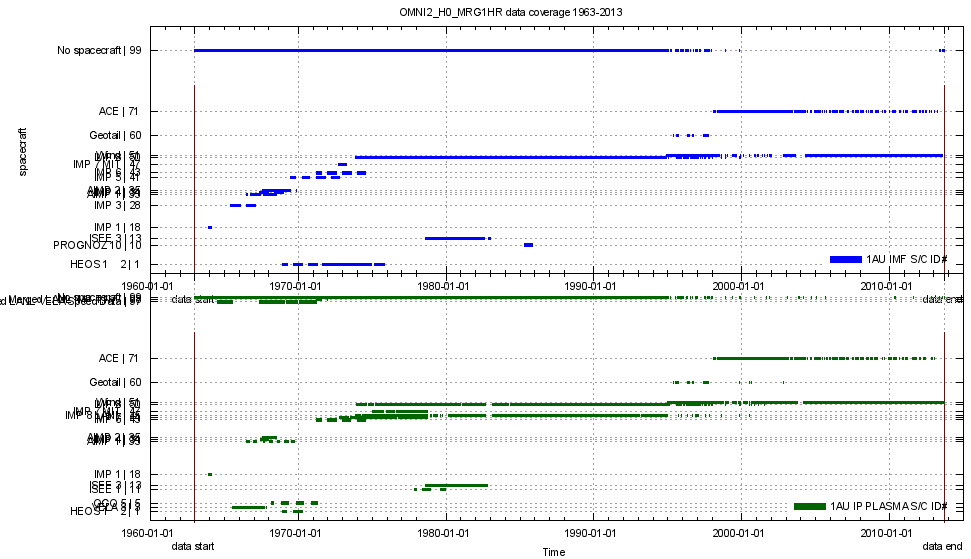
\includegraphics[width=0.5\textwidth]{images/gnuplots/omni_data_coverage_1963-2013_plot.png}
		\caption{OMNI intercalibrated multi-spacecraft data coverage per spacecraft. renew plot until 2016-12-31; integrate into 1 panel...}
	}{
		\label{fig:omni_data_coverage_1963-2013_plot}
	}
\end{figure}


\subsubsection{Advanced Composition Explorer}

s/c figure, launch date was 25 August 1997\\

MAG -- fluxgate magnetometer\\
SWEPAM\\	%https://sci-hub.ac/10.1023/A:1005040232597

data errors/gaps...\\

DSCOVR as replacement was launched on 11~Februar 2015. It is NOAA's SWPC real-time solar wind prime source since 27 July 2016.\footnote{\url{http://www.swpc.noaa.gov/products/real-time-solar-wind}}\\


\subsubsection{Solar Wind Structures}

Solar Wind Structures (SWS) list\\
derived by Richardson.... from OMNI data (only?)

permission received.\\

%http://cedarweb.vsp.ucar.edu/wiki/index.php/Tools_and_Models:Solar_Wind_Structures
characterization of near-Earth solar wind structures since 1963\\
SWS lists \citep{Richardson2000} and \citep{Richardson2012}


\subsection{Helios probes}
\label{sec:helios_probes}

see Helios data readme.txt\\
see paper\\

two different fluxgate magnetometers and a search coil magnetometer\\

see \autoref{fig:MPS_Helios}
\begin{figure}[htb]
	\begin{floatrow}
		\ffigbox[\FBwidth][]{
			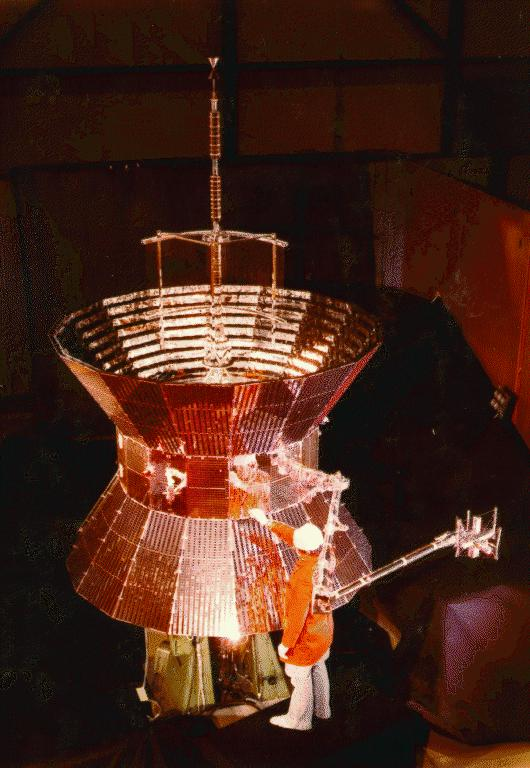
\includegraphics[width=0.3\textwidth]{images/MPS_Helios.jpg}
		}{
			\caption{One of the nearly identical twin Helios spacecraft. Credit: Max Planck Institute for Solar System Research. get permission...}
			\label{fig:MPS_Helios}
		}
		\ffigbox[\Xhsize]{
			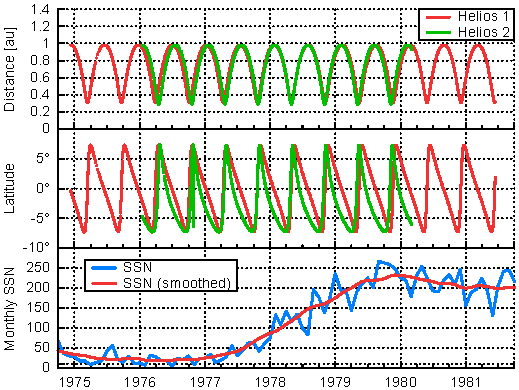
\includegraphics{images/gnuplots/Helios12_1h_r_b_ssn_plot.pdf}
		}{
			\caption{Plot of the Helios probes' solar distance and HGI latitude over their mission time, together with the monthly SSN and 13-month smoothed monthly SSN.}
			\label{fig:Helios12_1h_r_b_ssn_plot}
		}
	\end{floatrow}
\end{figure}

solar distance, HGI latitude and sunspot number during the Helios missions; see \autoref{fig:Helios12_1h_r_b_ssn_plot}\\

Helios orbit in the ecliptic plane and in the latitude polar plane (see \autoref{fig:Helios12_orbits_ecliptic_polar})\\
\begin{figure}[htb]
	\centering
	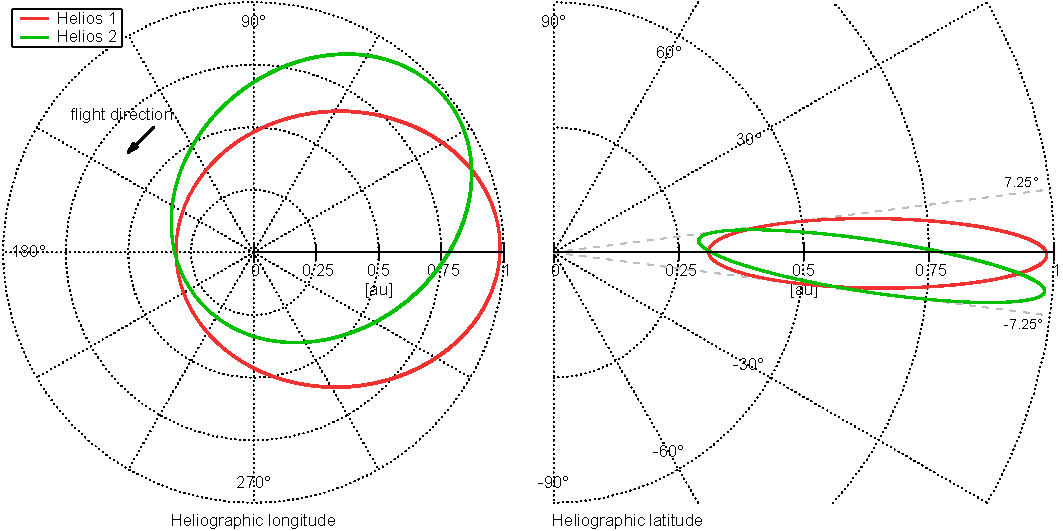
\includegraphics[width=\textwidth]{images/gnuplots/Helios12_orbits_ecliptic_polar.pdf}
	\caption{Helios orbits in the solar equatorial plane (left) and polar plane (right) (HGI-coordinates). change colors?}
	\label{fig:Helios12_orbits_ecliptic_polar}
\end{figure}

The Helios magnetic field and plasma data counts over solar distance are plotted in \autoref{fig:Helios12_1h_magswe_r-count_plot} and over latitude are plotted in \autoref{fig:latitude_frequency_plot}. build 2-panel figure...\\
\begin{figure}[htb]
	\begin{floatrow}
		\ffigbox{
			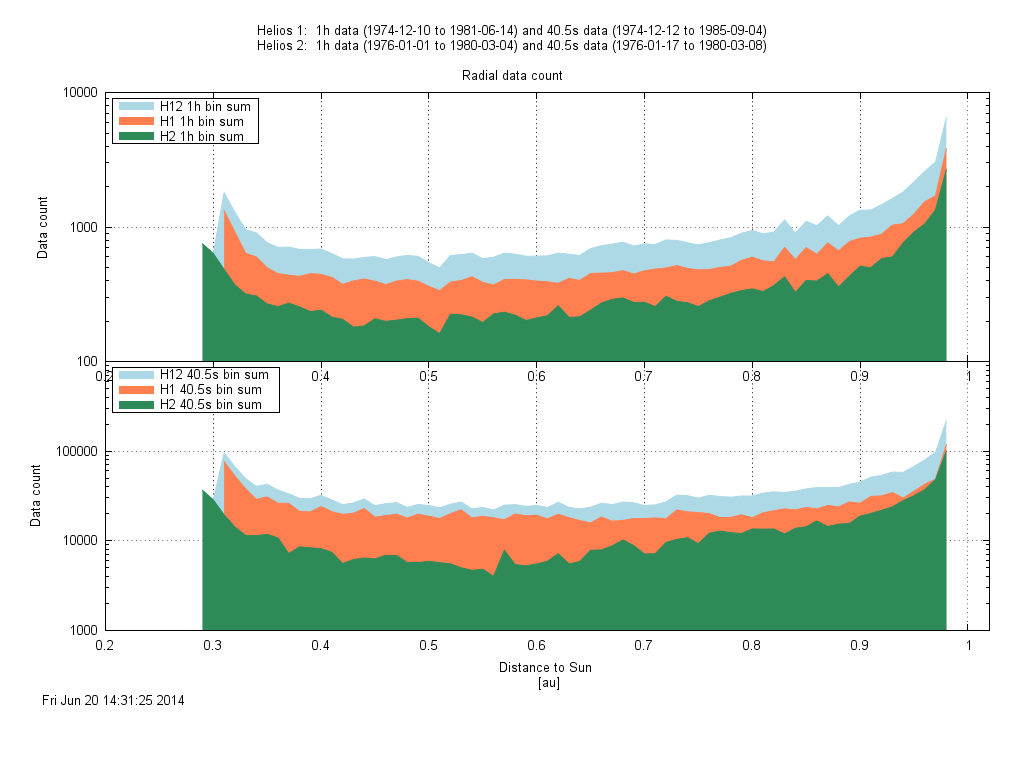
\includegraphics[width=0.45\textwidth]{images/gnuplots/Helios12_1h_magswe_r-count_plot.png}
		}{
			\caption{Plot of the Helios data count per 0.01~au solar distance bins. plot for mag and plasma individually..., combine with latitude plot...}
			\label{fig:Helios12_1h_magswe_r-count_plot}
		}
		\ffigbox{
			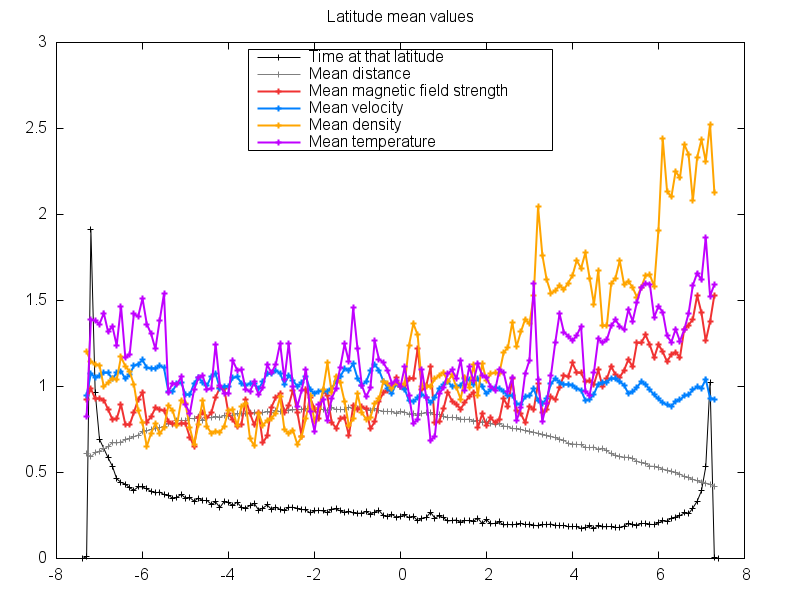
\includegraphics[width=\Xhsize]{images/gnuplots/latitude_frequency_plot.png}
		}{
			\caption{Plot of the Helios data count per 0.1° latitude. plot for mag and plasma individually... remove all other curves...}
			\label{fig:latitude_frequency_plot}
		}
	\end{floatrow}
\end{figure}

Solar wind data courtesy of R.~Schwenn, Max-Planck-Institut für Aeronomie, Lindau, magnetic field data courtesy of F.~Neubauer, Universität zu Köln. (see paper; into acknowledgements...)\\

%see presi 1.07 Inside Helios-Origins and Evolution-Salem.ppt
%see book Schwenn1990 https://books.google.de/books?id=W1DuCAAAQBAJ&printsec=frontcover&dq=Physics+of+the+Inner+Heliosphere+I.+Large-Scale+Phenomena&hl=de&sa=X&redir_esc=y#v=onepage&q=Physics%20of%20the%20Inner%20Heliosphere%20I.%20Large-Scale%20Phenomena&f=false



data sources -- see paper for replacing the following data\\
solar wind parameters: ACE, Helios, OMNI\\
geomagnetic indices: Kp, OMNI\\

Space Physics Data Facility (SPDF)\\

HELIOS 1 and 2 - orbital Parameters\\
\url{http://spdf.sci.gsfc.nasa.gov/pub/data/helios/helios1/traj/}\\
\url{http://spdf.sci.gsfc.nasa.gov/pub/data/helios/helios2/traj/}\\

Helios hourly merged mag \& plasma data:\\
HELIOS1\_COHO1HR\_MERGED\_MAG\_PLASMA\_2965.txt\\
HELIOS2\_COHO1HR\_MERGED\_MAG\_PLASMA\_3096.txt\\
\url{http://cdaweb.gsfc.nasa.gov}\\
temporal coverage of merged data\\
Helios 1: 1974-12-10 - 1981-06-14\\
Mag data availability: 42.6~\%\\
Plasma \& orbit data availability: 76.4~\%\\
Helios 2: 1976-01-01 - 1980-03-04\\
Mag data availability: 54.4~\%\\
Plasma \& orbit data availability: 91.8~\%\\


\subsection{Parker Solar Probe}
\label{sec:parker_solar_probe}

Sun angular diameter comparison, see presi S³\\
